\documentclass[12pt]{article}\usepackage[]{graphicx}\usepackage[dvipsnames]{xcolor}
% maxwidth is the original width if it is less than linewidth
% otherwise use linewidth (to make sure the graphics do not exceed the margin)
\makeatletter
\def\maxwidth{ %
  \ifdim\Gin@nat@width>\linewidth
    \linewidth
  \else
    \Gin@nat@width
  \fi
}
\makeatother

\definecolor{fgcolor}{rgb}{0.345, 0.345, 0.345}
\newcommand{\hlnum}[1]{\textcolor[rgb]{0.686,0.059,0.569}{#1}}%
\newcommand{\hlstr}[1]{\textcolor[rgb]{0.192,0.494,0.8}{#1}}%
\newcommand{\hlcom}[1]{\textcolor[rgb]{0.678,0.584,0.686}{\textit{#1}}}%
\newcommand{\hlopt}[1]{\textcolor[rgb]{0,0,0}{#1}}%
\newcommand{\hlstd}[1]{\textcolor[rgb]{0.345,0.345,0.345}{#1}}%
\newcommand{\hlkwa}[1]{\textcolor[rgb]{0.161,0.373,0.58}{\textbf{#1}}}%
\newcommand{\hlkwb}[1]{\textcolor[rgb]{0.69,0.353,0.396}{#1}}%
\newcommand{\hlkwc}[1]{\textcolor[rgb]{0.333,0.667,0.333}{#1}}%
\newcommand{\hlkwd}[1]{\textcolor[rgb]{0.737,0.353,0.396}{\textbf{#1}}}%
\let\hlipl\hlkwb

\usepackage{framed}
\makeatletter
\newenvironment{kframe}{%
 \def\at@end@of@kframe{}%
 \ifinner\ifhmode%
  \def\at@end@of@kframe{\end{minipage}}%
  \begin{minipage}{\columnwidth}%
 \fi\fi%
 \def\FrameCommand##1{\hskip\@totalleftmargin \hskip-\fboxsep
 \colorbox{shadecolor}{##1}\hskip-\fboxsep
     % There is no \\@totalrightmargin, so:
     \hskip-\linewidth \hskip-\@totalleftmargin \hskip\columnwidth}%
 \MakeFramed {\advance\hsize-\width
   \@totalleftmargin\z@ \linewidth\hsize
   \@setminipage}}%
 {\par\unskip\endMakeFramed%
 \at@end@of@kframe}
\makeatother

\definecolor{shadecolor}{rgb}{.97, .97, .97}
\definecolor{messagecolor}{rgb}{0, 0, 0}
\definecolor{warningcolor}{rgb}{1, 0, 1}
\definecolor{errorcolor}{rgb}{1, 0, 0}
\newenvironment{knitrout}{}{} % an empty environment to be redefined in TeX

\usepackage{alltt}
\usepackage{amsmath,amsfonts,amssymb,graphicx,authblk}
\usepackage[font={footnotesize,singlespacing},labelfont=bf]{caption}
\usepackage{titlesec,blkarray, bm} 
\usepackage{float,afterpage}
\usepackage[running,mathlines]{lineno}
\usepackage[vmargin=1in,hmargin=1in]{geometry}
\usepackage[authoryear,sort]{natbib}
\usepackage[dvipsnames]{xcolor}
\usepackage[nodisplayskipstretch]{setspace} 
\usepackage{hyperref}
\usepackage[section]{placeins}
\usepackage{gensymb}
\usepackage{enumitem}
\usepackage{orcidlink}
\usepackage{tabularx} % put this once in your preamble
\usepackage{booktabs}
\usepackage{pdflscape}  % or \usepackage{lscape}
%\usepackage{hyperref}
\setlist{topsep=.125em,itemsep=-0.15em,leftmargin=0.75cm}
\setlength{\parindent}{0.35in}

\usepackage[sc]{mathpazo} %Like Palatino with extensive math support
\usepackage[subtle]{savetrees}

\usepackage{lineno}
%\renewcommand{\refname}{Literature Cited}
%\renewcommand{\floatpagefraction}{0.9}
%\renewcommand{\topfraction}{0.99}
%\renewcommand{\textfraction}{0.05}

\clubpenalty = 10000
\widowpenalty = 10000

\sloppy 

\usepackage{ifpdf}
\ifpdf
\DeclareGraphicsExtensions{.pdf,.png,.jpg}
\usepackage{epstopdf}
\else
\DeclareGraphicsExtensions{.eps}
\fi

%\graphicspath{{/Users/jacobmoutouama/Dropbox/Miller Lab/github/endo-range-limits/Figure}}
%\graphicspath{{C:/Users/tm9/Dropbox/github/ELVI-endophyte-density/Figure}}
\newcommand{\tom}[2]{{\color{red}{#1}}\footnote{\textit{\color{red}{#2}}}}
\newcommand{\jacob}[2]{{\color{blue}{#1}}\footnote{\textit{\color{blue}{#2}}}}
\renewcommand\Authfont{\normalfont\normalsize}    % sets author names to small
\renewcommand\Affilfont{\normalfont\small} % sets affiliations even smaller
\setlength{\affilsep}{1em}  
%\doublespacinq



% I cannot get \orcidlink working on my computer so for now replacing this with \textit

%-------------------------------------------------------------------------
\title{\Large When Mutualism Becomes Costly: Abiotic Stress Shapes Grass Demography}
\author[1,2,3]{Jacob K. Moutouama\,\orcidlink{0000-0003-1599-1671} \thanks{Corresponding author: jmoutouama@gmail.com}}
\author[1]{Julia Martin}
\author[1]{Alexandra Jimenez Martín}
\author[1,4]{Josh Fowler}
\author[1]{Ali Campbell}
\author[1]{Chris Oxley}
\author[1]{Karl Schrader}
\author[1]{Tom E.X. Miller\,\orcidlink{0000-0003-3208-6067}}
\affil[1]{Program in Ecology and Evolutionary Biology, Department of BioSciences, Rice University, Houston, TX USA}
\affil[2]{Department of Botany, University of British Columbia, Vancouver, BC, Canada}
\affil[3]{Biodiversity Research Centre, University of British Columbia, Vancouver, BC, Canada}
\affil[4]{University of Miami, Department of Biology, Miami, FL USA}
\date{} % clear date
%\renewcommand\Authands{ and }

\sloppy

%-------------------------------------------------------------------------
\IfFileExists{upquote.sty}{\usepackage{upquote}}{}
\frenchspacing
\begin{document}
%\SweaveOpts{concordance=TRUE}
\renewcommand{\baselinestretch}{1.2}
\maketitle
% \bigskip 
%45 character limit on running head
\noindent\textbf{Running header:} Stress and Grass–Endophyte Interactions
\bigskip 

\noindent\textbf{Keywords:} demography, mutualism, parasitism, plant–fungi interactions, range limits, stress gradient hypothesis

\bigskip 
\noindent\textbf{Submitted to:} \textit{Ecology letters} (Letter)

\bigskip 
\noindent\textbf{Data accessibility statement:} 
If the paper is accepted, all data and computer scripts supporting the results will be archived in a Zenodo package, with the DOI included at the end of the article. 
During peer review, our code (Stan and R) is available at \url{https://github.com/jmoutouama/endo-range-limits}. 

\bigskip 
\noindent\textbf{Conflict of interest statement:} None.

\bigskip
\noindent\textbf{Authorship statement:}
%J.K.M., A.C. and T.E.X.M. designed the study.
%A.C. and T.E.X.M. collected the data. 
%All authors conducted the statistical analyses and modeling.
%J.K.M. drafted the manuscript, and T.E.X.M contributed to revisions.

\bigskip
\noindent\textbf{Abstract:}\\
\noindent\textbf{Main Text:}\\
\noindent\textbf{Figures: 6}\\
\noindent\textbf{Tables: X}\\
\noindent\textbf{References: X}

\newpage
%\SweaveOpts{concordance=TRUE}
\linenumbers
%-------------------------------------------------------------------------
\spacing{1.25}
\section*{Abstract}
%150 words limit for Ecology letter. The number now is 150
Beneficial interactions between plants and fungi are ubiquitous and foundational to terrestrial ecosystems.
Plant-fungal mutualisms are expected to strengthen under environmental stress, yet the relative importance of abiotic and biotic factors in eliciting mutualistic benefits remains unclear.
We studied how the demographic effects of seed-transmitted fungal endophytes on native three grass host species varied in response to abiotic and biotic factors using geographically distributed field experiments along an aridity gradient, cross with herbivore access or exclusion. 
Vital rate models showed that all components of host fitness (survival, growth and fertility) declined with increasing, indicating reduced performance under abiotic stress. 
Declines were more pronounced in individuals hosting endophytes, suggesting that interactions that are beneficial under benign conditions can become costly under abiotic stress. 
On the other hand, herbivory had no detectable effect on host demography or on the demographic effects of hosting endophytes. 
Our results indicate that abiotic stress was the primary determinant of interaction outcomes between plants and fungal symbionts, but in the opposite direction as predicted by theory and prior work. 
These results highlight that symbiotic fungi can become liabilities under stress, with implications for the dynamics of plant-fungal mutualisms under global change.
%--------------------------------------------------------------------
\newpage
\section*{Introduction}
Plant-microbe symbioses are widespread and ecologically important. 
These interactions are famously context-dependent, where the direction and strength of the interaction outcome depend on the environment in which it occurs \citep{hoeksema2015context, bronstein1994conditional}.
For example, plant-microbe  interactions that are beneficial under stressful conditions  may become neutral or parasitic under benign conditions \citep{giauque2019endophyte}. 

Stress may derive from biotic and/or abiotic factors. 
Under biotic stress, such as herbivory, microbial symbiosis can benefit host plants by facilitating the production of secondary compounds that deter feeding or exert direct toxicity, thereby reducing herbivore growth, survival, and oviposition \citep{atala2022fungal,bastias2017epichloe,vega2008insect}. 
Similarly under abiotic stress, such as low precipitation or high temperature, \tom{symbionts can increase their host tolerance \citep{clay2002evolutionary}}{Can you expand this a bit? The previous sentence gave a more thorough explanation of how symbionts can benefit hosts exposed to herbivory. How do symbionts promote tolerance of abiotic stress? Through this section, keep the scope pretty wide, so don't just focus on the grass-endophyte literature.}.
\tom{Mycorrhizal fungi form extensive networks that increase root surface area, helping plants absorb more water and nutrients such as phosphorus and nitrogen \citep{amijee1989development}. }{Unclear how this relates to the preceding sentences. Is this meant to be an example of how symbionts promote tolerance of abiotic stress? If so, it does not come through clearly. What is the importance of access to phosphorous and nitrogen, and how does this related to abiotic stress?}
Symbiotic microbes can also stimulate plants to produce antioxidant enzymes like superoxide dismutase and catalase that reduce oxidative damage caused by stresses such as drought, salinity, and heat \citep{ruiz1996superoxide}.
All these mechanisms could help the host species better buffer against environmental stochasticity \citep{fowler2023geographic}.

\tom{In resource-limited environments, maintaining symbionts can also impose significant costs on hosts \citep{johnson1997functioning, bronstein2001exploitation}. }{You are introducing a new idea, so I suggest starting a new paragraph with a strong topic sentence, and more fully developing the idea of costs of symbiosis.}
Because microbes depend on host-derived carbon and nutrients, plants must allocate part of their limited resources to sustaining the symbiont.
This investment can reduce host growth, reproduction, or competitive ability, particularly when the benefits provided by the symbiont do not outweigh these costs \citep{klironomos2003variation}. 

%\tom{However, in many plant-microbe interactions, host protection is not guaranteed solely by the presence of a symbionts; rather, the density of the symbiont can determine the effectiveness of this protection \citep{laughton2014combined}. 
%Higher endophyte densities may lead to increased resource exploitation by the symbiont, potentially imposing costs on the host, such as reduced growth or reproduction \citep{faeth2009asexual}.}{I like these sentences and the idea is really interesting and important -- but if we are not using the endo density data in this paper then I would remove.}
%This cost is often manifested by a reduction in host biomass or reproductive success \citep{faeth2009asexual}, particularly under harsh abiotic conditions \citep{cui2024review}. 
%Ultimately, these context-dependent costs and benefits may underlie the observed distribution of host species.

\tom{Context-dependence}{What is the topic of this paragraph, and what is it intended to do differently than the preceding paragraphs? A lot of this material overlaps heavily with what you have already presented above. Think about the logic structure that you want for the intro, and make sure your paragraphs are taking readers through a logical progression of ideas.} raises the hypothesis that plant–microbe interactions are likely to vary across abiotic stress gradients, such as high temperatures or low precipitation, as well as under biotic stressors like herbivory, with significant implications for host fitness in variable environments. 
\tom{If microbial symbiosis provides greater benefits under these stressful conditions, symbionts could enhance host survival, growth, and reproduction.}{Statements like this are a little circular (``if symbionts are beneficial then the plant would benefit.'') Can you sharpen this?} \citep{allsup2023shifting,rudgers2020climate}. 
For example, fungal endophytes of grasses enhance host tolerance to abiotic stress in \emph{Bromus laevipes} by improving population survival in dry environments \citep{david2019soil,afkhami2014mutualist}.
Even when symbionts do not directly increase survival under stress, they may still promote host fitness by enhancing growth and reproduction, thereby offsetting the negative effects of lower survival rates \citep{yule2013costs}. 
\tom{Conversely, if microbial symbiosis becomes costly under stressful conditions, symbionts could reduce host fitness}{Also circular.} \citep{benning2021microbes,benning2021plant,bennett2022costs}. 
For instance, mycorrhizal fungi require substantial carbon subsidies from the host plant (up to 20\% of photosynthetically fixed carbon) \citep{thirkell2020carbon,soudzilovskaia2015quantitative}. 
When photosynthesis is limited by abiotic stress, this carbon cost may outweigh the benefits of symbiosis, leading to reduced host fitness.

%Mutualist limitation reduces population fitness and therefore limits range expansion in \emph{Medicago polymorpha} populations \citep{lopez2021microbial}. 
%Although context dependence, along with spatiotemporal variations in abiotic environmental conditions may reduce the effectiveness of the benefits provided by the symbiont to the host species, our understanding of the mechanisms that alter host-symbiont interactions across species geographic range remains limited.

%\tom{Despite growing interest in the ecological and evolutionary roles of symbiosis, most studies focus on the host plant’s perspective and rarely manipulate symbiont prevalence to evaluate how environmental variation shapes the symbiont’s effects on host demography across geographic ranges. 
%Yet, symbionts promote their own fitness by influencing host life history traits and enhancing resistance to stress \citep{kazenel2015mutualistic, giauque2019endophyte, saikkonen1998fungal}. 
%Theory predicts that exclusive vertical transmission fosters mutualism and leads to high symbiont prevalence in host populations \citep{fine1975vectors}. 
%Field studies suggest that, under stressful conditions, beneficial symbionts may increase in prevalence and even reach fixation if their fitness advantages outweigh reproductive costs \citep{donald2021context}. 
%However, populations with lower prevalence may experience higher symbiont loss among offspring \citep{afkhami2008symbiosis}. 
%Thus, overlooking symbiont dynamics could result in inaccurate predictions of host population responses to global change.}{Again, I really like this paragraph, but we need to think about whether and how the symbiont density data will be used here. Is that what you are pointing towards here? Otherwise I am not sure why you are bringing up symbiont prevalence, since I did not think the prevalence data were going into this paper.}

Despite growing interest in the role of symbiosis in host performance, few studies have examined under natural conditions how both abiotic and biotic stressors shape the effects of symbionts on host demography along stress gradients \citep{louthan2015and}. 
Moreover, it remains unclear which stressor is most critical in eliciting the benefits of \tom{endophyte symbiosis}{What is the intended scope at this point in the paper? Is this meant to be a general statement about microbial symbioses, or are we now talking specifically about Epichloe symbioses in grasses? I think the Intro can provide clearer sign-posting for this. There is a lot of literature on drought and herbivory in the Epichloe literature. I think it would be good to have a paragraph late in the Intro that introduces this system and briefly covers the literature on drought and herbivory, highligting that few (or no?) previous studies have looked at both.}, or how multiple stressors may interact to influence host demography. 
Herbivory is a biotic factor that can significantly affect host fitness \citep{benning2019biotic} and mediate the outcomes of symbiotic interactions. 
Herbivores reduce host fitness through tissue damage, defoliation, and altered resource allocation \citep{maron2006herbivory}, and can also impose indirect ecological costs by influencing reproductive or growth strategies \citep{miller2008herbivore}. 
These ecological costs may shape the selective landscape in ways that favor symbiont persistence or transmission \citep{clay2005herbivores}. 
For example, herbivory can enhance the fitness benefits of endophyte infection by triggering host defense pathways or promoting vertical transmission of the symbiont \citep{gundel2020simulated,agrawal1999transgenerational}. 
If the ecological context of herbivory alters the net fitness effects of symbiosis, then interactions between herbivory and abiotic stress (e.g., drought or high temperature) may play a critical role in determining host population persistence.\tom{}{The opening sentence suggested that this paragraph would be about the combined and relative roles of abiotic and biotic stress, but most of this paragraph is actually about herbivory. Again, bring attention to the way you structure paragraphs. Use clear topic sentences, and make sure the content of the paragraph stays true to the topic sentence. }

\tom{}{Here is where I might dedicate a paragraph to describing the biology and context-dependence of the grass-endophyte symbioses.}

Working across an aridity gradient in the south-central US, we investigated how endophyte symbiosis influences \tom{host-plant demography under varying abiotic stress}{This paper includes multiple vital rate responses, and it might be strategic to highlight in the Intro the value of looking at multiple vital rates, since they may respond differently to abiotic or biotic stress (I am thinking of the demographic compensation ideas).}. 
This region provides an ideal system to study biologically realistic stress gradients because it spans a strong east–west precipitation gradient, with mesic conditions in the east transitioning to increasingly arid conditions in the west. 
At each site along the gradient we also tested herbivory as a biotic stressor to evaluate its potential interactive effects with abiotic conditions. 
Specifically, we studied the symbiotic association between three native cool-season grass species (\emph{Agrostis hyemalis}, \emph{Elymus virginicus}, and \emph{Poa autumnalis}) and their vertically transmitted fungal symbionts (\emph{Epichloë} spp.). 
Our experiment was designed to address the \tom{following questions}{I think these questions can be improved but I will keep working through the methods and results, then return to this.}:
\begin{enumerate}
    \item Under combined abiotic stress and herbivory, do endophytes provide fitness benefits or impose costs on their host plants?
    \item Between abiotic and biotic factors, which plays a stronger role in \tom{shaping host population demography in association with endophytes}{This is vague. Can you articulate this question more precisely?}?
\end{enumerate}
\tom{We hypothesized...}{Could be here or elsewhere, but I recommend including hypotheses or predictions toward the end of the Intro. Readers will need to know what to look for in the results. This occurred to me when I got to the methods section about modeling effects aridity, herbivory, and symbiosis. There is not enough provided here to anticipate what types of analyses you would need to do, and what your expectations would be. So that is the main point of this comment: set up expectations for readers.}

%\begin{enumerate}
%    \item Because endophytes often produce defensive compounds (e.g., alkaloids), plants with endophytes will experience less herbivore damage and maintain higher vital rate compared to plants without endophytes  \tom{when grazed}{We do not have much direct information about `grazing'. I would keep the focus on herbivore access or exclusion, since that is what we directly measured.}.
%    \item Because endophytes can improve \tom{drought tolerance}{I would lead with the abiotic stressors, since that is more central to the experimental design.} (e.g., by enhancing water use efficiency or root growth), plants with endophytes will outperform plants without endophytes more in dry conditions than in wet conditions.
%     \item The combined stresses of herbivory and low precipitation will create conditions where the mutualistic benefits of endophytes are most pronounced, giving plants with endophytes a strong performance advantage over plants without endophytes.
%     \item The combined stresses of herbivory and low precipitation will amplify the physiological demands on the host plant, \tom{such that the additional resource costs of maintaining endophyte associations will  reduce overall plant performance resulting in endophyte-infected plants performing worse than uninfected plants under extreme stress conditions}{I am confused here because this prediction seems to contradict the preceding prediction. But either way, I still think it would be more compelling to phrase these as questions.}.
%\end{enumerate}
%--------------------------------------------------------------------
\section*{Materials and methods}
\subsection*{Study system}
Our study focused on three cool-season perennial grasses native to woodland and prairie habitats of eastern North America: \emph{Agrostis hyemalis}, \emph{Elymus virginicus}, and \emph{Poa autumnalis} (subfamily Pooideae) \citep{shaw2011guide}.
\emph{A. hyemalis} is a small, short-lived perennial that germinates from autumn to late winter and typically flowers between March and July. \emph{E. virginicus} is a larger, long-lived species that begins flowering as early as March or April and continues throughout the summer. \emph{P. autumnalis} has a similar growth form to \emph{E. virginicus} and flowers from late spring through summer.
All three species host \emph{Epichloë} fungal endophytes, which are primarily transmitted vertically through seeds. 
\emph{Agrostis hyemalis} is associated with \emph{Epichloë amarillans} \citep{white1994endophyte}, \emph{E. virginicus} typically hosts \emph{Epichloë elymi} \citep{liu2023fungi}, and \emph{P. autumnalis} can also harbor endophyte taxa capable of horizontal transmission via sexual stromata on inflorescences or asexual conidia on leaf surfaces \citep{clay2002evolutionary, gundel2020simulated,leuchtmann2014nomenclatural}. 
Horizontal transmission is rare, influenced by environmental and genetic factors, and was not observed in our study system.
To examine the effects of endophytes on host species across a stress gradient, we established eight plots (1.5 m $\times$ 1.5 m) at each of seven sites along an aridity gradient in Louisiana and Texas (Fig.~\ref{fig:site}A-D). 
Each plot contained 15 individuals of a single species, with half of the plots protected from herbivores using exclusion cages to assess the interactive effects of endophytes and herbivory (Fig.~\ref{fig:site}E).
In summer–fall 2021, seeds were collected from naturally symbiotic source populations and either heat-treated to remove endophytes or left untreated, producing symbiont-free ($E^-$) and symbiotic ($E^+$) plants from the same genetic lineages.

\subsection*{Source populations and symbiont removal}
Plants used in the common garden experiment were derived from natural (source) populations throughout the natural distribution of the species (Fig.~\ref{fig:site},Table~\ref{tab:source_pop}). 
Seeds were collected from these source populations, and some were heat-treated at 60°C for approximately five days (120 hours) to produce endophyte-negative plants ($E^-$), a method that eliminates endophytes without affecting seed viability. 
All seeds, both heat-treated and non-heat-treated, were planted in the Rice University greenhouse, where seedlings were fertilized every two weeks. 
Seedlings were then vegetatively propagated to produce enough individuals for the experiment. 
Before field planting, we confirmed endophyte status ($E^+$ or $E^-$) of all seedlings using either microscopy or an immunoblot assay. 
Leaf tissues were stained with aniline blue lactic acid and viewed under a compound microscope at 200x–400x to identify fungal hyphae. 
The immunoblot assay (Phytoscreen field tiller endophyte detection kit, Agrinostics Ltd. Co.) uses monoclonal antibodies that target proteins of \emph{Epichloë} spp. and a chromagen to visually indicate presence or absence.
Both methods yield similar detection rates.

\subsection*{Common garden experimental design}
We conducted our common experiment across spanning the precipitation gradient from Louisiana to central Texas, USA (Fig.~\ref{fig:site}, Table~\ref{tab:exp_sites}). 
During our study period (2023-2025) realized precipitation at these sites corresponded well to 30-year normals, with wetter eastern sites and drier western sites. 
%Louisiana represents mesic conditions, whereas Texas experiences increasingly arid conditions, making this gradient an ideal natural laboratory to study the effects of precipitation and aridity on plant–microbe interactions.  
Mean annual temperature did not differ significantly across sites (Fig.~\ref{Sup:temp}), so we focus on precipitation as the primary abiotic factor that varied across sites.  
This gradient also overlaps and exceeds the natural distributions of our focal species, ensuring realistic exposure to climatic and biotic conditions (Fig.~\ref{fig:site}).  

Plots were randomly assigned one of four initial endophyte frequency treatments (80\%, 60\%, 40\%, or 20\%) and one of two herbivore access treatments (fenced to exclude herbivores or unfenced to allow access). In the fenced plots, insecticides were applied periodically to eliminate small herbivorous insects, as \emph{Agrostis hyemalis}, \emph{Epichloë amarillans}, and \emph{Poa autumnalis} are naturally subject to herbivory by both insects and larger mammals.
To ensure that our herbivory treatment reflected the level of herbivory experienced by individual plants, we counted the number of damaged plants per plot and estimated the proportion of damaged plants per site and herbivore treatment. 
Our results confirmed that the herbivory treatment was effective (Fig.~\ref{fig:site}F).

\begin{figure}[H]
\centering
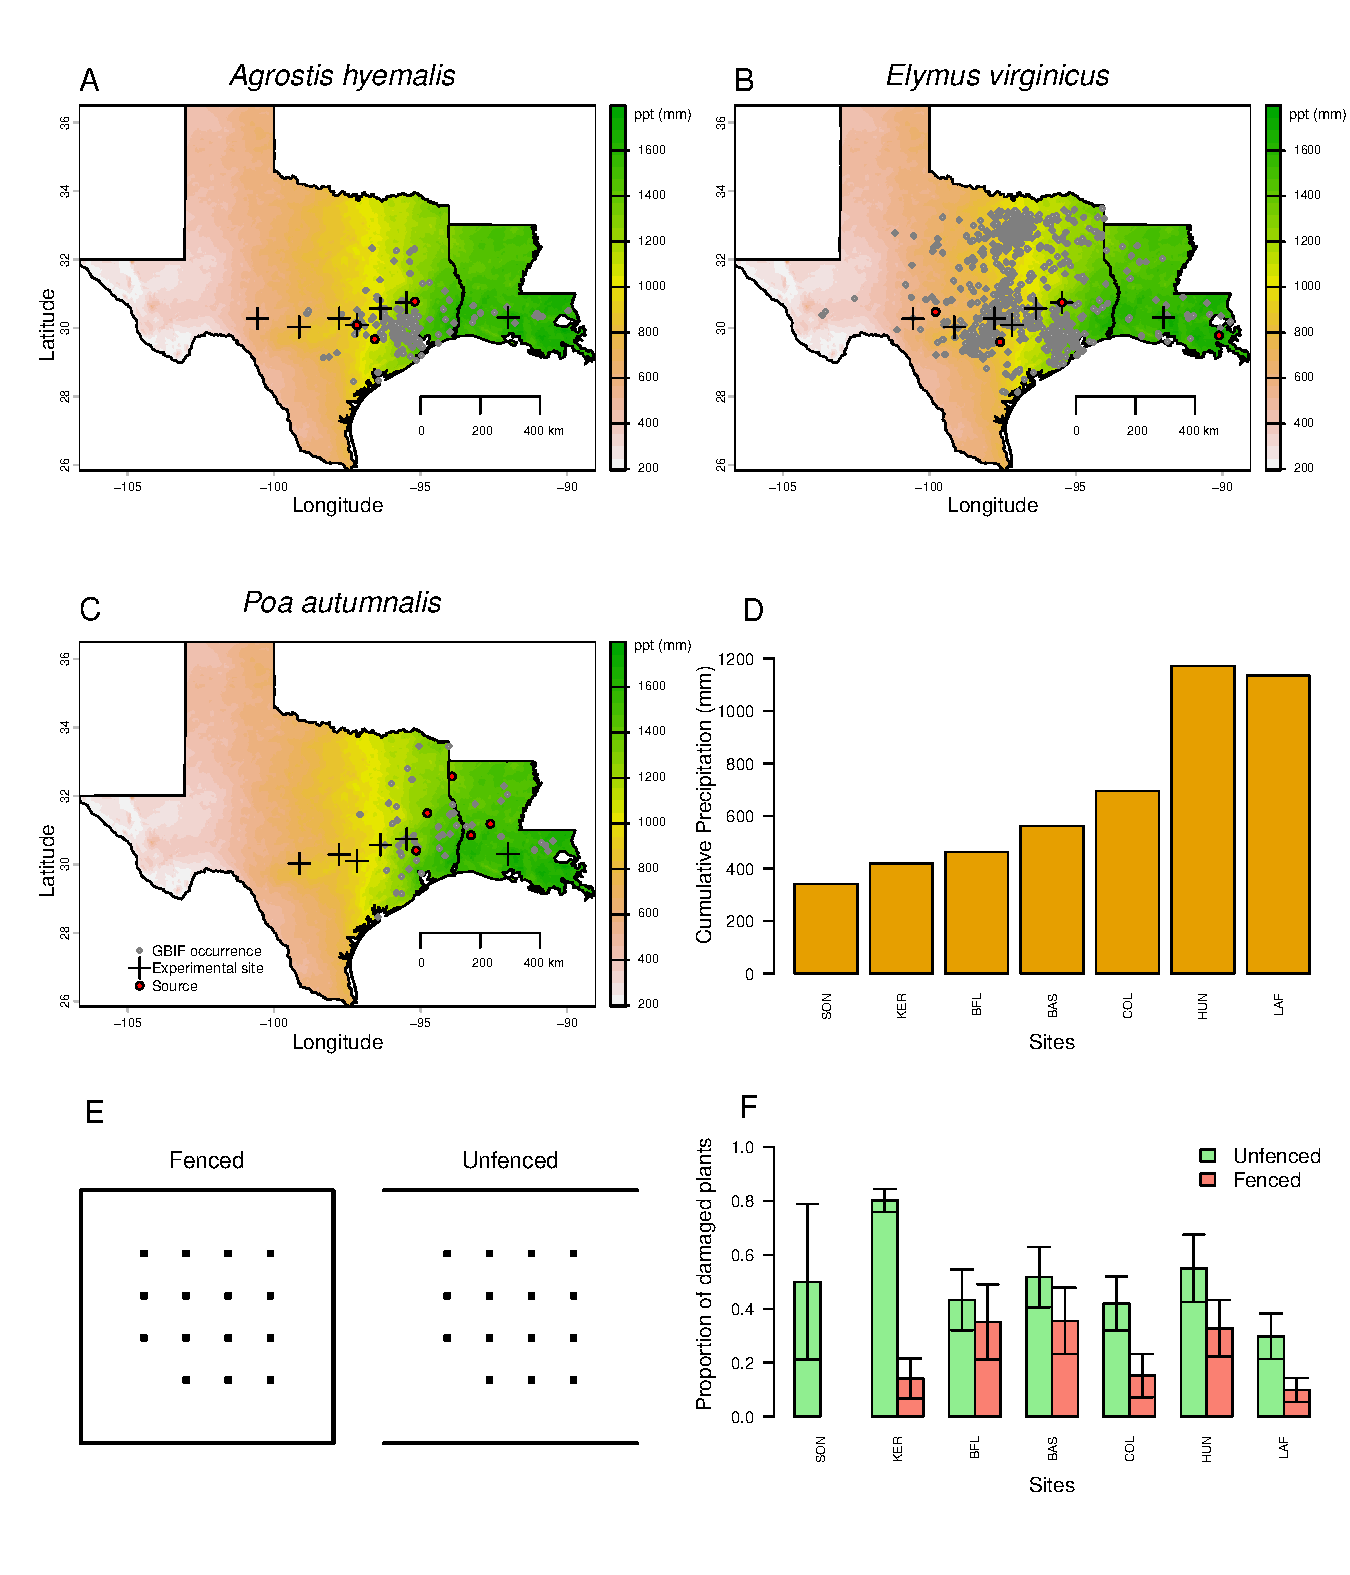
\includegraphics[width=1\textwidth]{../Figure/clim_map.pdf}
\caption{Distribution of common garden sites along a natural aridity gradient from Texas to Louisiana, US for (A) \emph{Agrostis hyemalis}, (B) \emph{Elymus virginicus}, and (C) \emph{Poa autumnalis}. 
Climate data in A–C are based on 30-year normals of climate predictions (1993–2023) from PRISM data \citep{PRISM2024}, which illustrate the precipitation gradient across sites (scale on the right is in mm. 
Red dots indicate the locations of source populations, while grey dots represent Global Biodiversity Information Facility (GBIF) occurrence records for each species within the study area \citep{gbif2025_aghy,gbif2025_elvi,gbif2025_poau}.
D) Cumulative precipitation during the study period (May 2023 – June 2025) at each site, ordered west to east. Values are also derived from PRISM climate data \citep{PRISM2024}.}
\label{fig:site}
\end{figure}

\subsection*{Demographic data collection}
We collected demographic data, including survival, growth, and reproduction, during the flowering season of each species: \emph{Agrostis hyemalis} and \emph{Poa autumnalis} were censused in May, and \emph{Elymus virginicus} was censused in June of 2023, 2024, and 2025.
For each individual, plant survival was recorded as alive or dead and, for surviving plants, size was measured as the number of tillers.  
We recorded the number of inflorescences per plant for all three species and counted the number of spikelets on up to three inflorescences from reproducing individuals of \emph{Poa autumnalis} and \emph{Elymus virginicus}.
%Spikelet counts were limited to three reproducing tillers per plot due to the time-consuming nature of this measurement.  

\subsection*{Modeling the effects of aridity, herbivore exclusion, and symbiosis on grass demography}
To quantify how abiotic stress and herbivore exclusion (as a proxy for herbivory pressure) modify the demographic outcomes of plant–fungal interactions, we developed hierarchical models for survival, growth, and fertility.
Survival was modeled with a Bernoulli distribution, growth with a Gaussian distribution, and fertility with the number of inflorescences per plant, and for \textit{E. virginicus} and \textit{P. autumnalis}, the number of spikelets with negative binomial distributions. 
Growth was quantified as the log ratio of the number of tillers between consecutive censuses (i.e., $\log(\text{tiller}_{t+1}/\text{tiller}_{t})$) for plants that were alive in both years.
We modeled all vital rates (survival, growth, and fertility) using species-specific fixed effects for symbiosis (endophyte presence), precipitation, and herbivore access, including all relevant two- and three-way interactions. Each observation $i$ corresponds to a plant in a given year; individuals can appear in multiple years. For simplicity, we omit the full subscript notation for species, plot, population, and site-year in the following equation, which is explicitly included in the Stan model:

\begin{equation}\label{eq:full_model}
\begin{aligned}
\mu_i &= \beta_0[Sp_i] + \beta_P[Sp_i] P_i + \beta_{P^2}[Sp_i] P_i^2 + \beta_{endo}[Sp_i]\, endo_i + \beta_{herb}[Sp_i]\, herb_i \\
&\quad + \beta_{endo \times P}[Sp_i]\, endo_i P_i 
       + \beta_{endo \times P^2}[Sp_i]\, endo_i P_i^2 
       + \beta_{herb \times P}[Sp_i]\, herb_i P_i \\
&\quad + \beta_{herb \times endo}[Sp_i]\, herb_i endo_i + \beta_{endo \times herb \times P}[Sp_i]\, endo_i herb_i P_i \\
&\quad  + \phi_{\text{site}[i],Sp_i} 
       + \omega_{\text{source}[i],Sp_i} 
       + \rho_{\text{plot}[i],Sp_i} .
\end{aligned}
\end{equation}

\noindent Here, $P_i$ is total precipitation (mm) averaged over the 12 months preceding the census, $endo_i$ indicates endophyte presence, and $herb_i$ indicates herbivore access.
Random effects account for background variation at multiple hierarchical levels: $\phi_{\text{site}[i],Sp_i}$ captures site-to-site heterogeneity not explained by precipitation, $\omega_{\text{source}[i],Sp_i}$ captures variation associated with the provenance of transplants, and $\rho_{\text{plot}[i],Sp_i}$ captures plot-to-plot variation.
Each species has its own random effect for each site, source, and plot, while the variance parameters ($\sigma_{\text{site}}$, $\sigma_{\text{source}}$, $\sigma_{\text{plot}}$) are shared across species. 
This hierarchical structure allows the model to ``borrow strength'' across species, improving estimates of fixed effects and background variation, while still capturing species-specific responses to environmental heterogeneity.
We confirmed that models effectively captured key aspects of the grass demography data, including means, standard deviations, and quantiles  using a posterior predictive check (Fig.~\ref{sup:ppc_vital}).

\subsection*{Disentangling abiotic and biotic drivers on cool-season grass demography}
To understand whether biotic or abiotic stressors are more important for the benefits of the symbiosis, we developed three candidate models for each vital rate: (1) endophyte × precipitation, (2) endophyte × herbivory, and (3) endophyte × precipitation × herbivory, which allows for additive and interactive effects of abiotic and biotic factors. 
Abiotic effects were represented by precipitation, while biotic effects included herbivory. 
All models followed the hierarchical structure described above, differing only in the inclusion of predictor terms (Supplementary Method \ref{sec:models}).
For each vital rate, we determined the best-supported model using leave-one-out cross-validation (LOOCV) \citep{vehtari2017practical}. 
LOOCV iteratively holds out one observation as a test set while fitting the model on the remaining $n-1$ observations. 
This process is repeated $n$ times, resulting in $n$ fitted models. 
The overall test error for each vital rate was estimated by averaging the prediction errors across the $n$ models:
\begin{align}\label{eq:Loo}
CV_{n} = \frac{1}{n} \sum_{i=1}^{n} (y_{i} - \hat{y}_{i})^2.
\end{align}

All models were implemented in R \citep{RCoreTeam} using Stan via the \texttt{rstan} interface \citep{Rstan}.


%%%%%%%%%%%%%%%%%%%%%
% Acknowledgments
%%%%%%%%%%%%%%%%%%%%%
% You may wish to remove the Acknowledgments section while your paper 
% is under review as the Acknowledgments may reveal your identity.
% If you remove this section, you will need to add it back in to your
% final files after acceptance.
\section*{Results}
\subsection*{Endophyte presence influenced host survival and reproduction across the abiotic stress gradient, with no effects of herbivory}
Survival declined under lower precipitation, and the effect of endophytes on survival changed from beneficial under wetter conditions to costly under drier conditions (Fig.~\ref{fig:Surv}; Fig.~\ref{sup:survival_delta}; Table~\ref{tab:delta_summary_surv}). 
For \textit{Agrostis hyemalis} and \textit{Elymus virginicus}, endophytes generally enhanced survival under wetter conditions (median $\Delta$~(E$^{+} - $E$^{-})$ increased from $\sim$0.004 and 0.023 at $\sim$1113 mm to 0.033 and 0.084 at $\sim$2163 mm, respectively, with posterior probabilities Pr ($\Delta>0$) $>$ 0.55 and $>$0.84), and became neutral or slightly negative under drier conditions ($\sim$0.007 and $-$0.013 at $\sim$766 mm, Pr ($\Delta>0$) $\sim$0.12--0.43). 
In contrast, \textit{Poa autumnalis} exhibited divergent endophyte effects depending on herbivore exclusion: in fenced plots (herbivores excluded), endophytes generally enhanced survival across the precipitation gradient (median $\Delta \sim$0.005--0.027, Pr ($\Delta>0$) $\sim$0.64--0.69), whereas in unfenced plots (herbivores had access), endophytes had a negative effect on survival (median $\Delta \sim -0.012$ to $-0.052$, Pr ($\Delta>0$) $\sim$0.17--0.25).

Endophytes consistently enhanced growth for \textit{Agrostis hyemalis} and \textit{Elymus virginicus}, whereas their effects on \textit{Poa autumnalis} depended strongly on herbivore access (Fig.~\ref{fig:growth}; Fig.~\ref{sup:growth_delta}; Table~\ref{tab:delta_summary_grow}). 
For both \textit{Agrostis hyemalis} and \textit{Elymus virginicus}, endophyte effects were positive across the entire precipitation gradient, with $\mathrm{Pr}(\Delta > 0)$ consistently above 0.91. 
Median $\Delta$~(E$^{+} - $E$^{-})$ ranged from 0.3972 to 0.4259 for \textit{A.~hyemalis} and from 0.2673 to 0.2521 for \textit{E.~virginicus}, indicating persistent growth benefits under both dry and wet conditions. 
In contrast, \textit{Poa autumnalis} showed opposing responses depending on herbivore access: endophytes tended to increase growth in fenced plots (median $\Delta \sim$0.0181--0.3338, $\mathrm{Pr}(\Delta > 0) \sim$0.55--0.91) but had neutral to slightly negative effects in unfenced plots (median $\Delta \sim$--0.1283 to 0.0688, $\mathrm{Pr}(\Delta > 0) \sim$0.30--0.65).


Endophyte-mediated effects on flowering output were generally positive for \textit{Agrostis hyemalis} and \textit{Poa autumnalis}, but varied with precipitation and herbivore access for \textit{Elymus virginicus} (Fig.~\ref{fig:flowering}; Fig.~\ref{sup:flowering_delta}; Table~\ref{tab:delta_summary_flow}). 
For \textit{Agrostis hyemalis} and \textit{Poa autumnalis}, endophyte infection generally enhanced flowering across the entire precipitation gradient. 
In \textit{Agrostis hyemalis}, median $\Delta$~(E$^{+} - $E$^{-})$ increased modestly from approximately 0.0161 at $\sim$1316~mm to 0.0178 at $\sim$2163~mm under unfenced conditions, and from 0.0171 to 0.0164 under fenced conditions, with $\mathrm{Pr}(\Delta > 0)$ consistently between 0.66 and 0.77, indicating a consistent though moderate benefit. 
Similarly, \textit{Poa autumnalis} showed strong and positive endophyte effects on flowering, especially under herbivore exclusion, where median $\Delta$ rose from 0.0760 at $\sim$774~mm to 0.1621 at $\sim$1316~mm and remained high at wetter sites ($\mathrm{Pr}(\Delta > 0) > 0.99$). 
In contrast, \textit{Elymus virginicus} exhibited a precipitation-dependent response: while endophyte infection slightly enhanced flowering at higher precipitation (median $\Delta \sim$0.0178–0.0436, $\mathrm{Pr}(\Delta > 0) \sim$0.63–0.78), it imposed a cost under drier conditions, where median $\Delta$ values were near zero or negative (–0.0141 to 0.0067, $\mathrm{Pr}(\Delta > 0) \sim$0.42–0.55). 

Endophyte effects on spikelet production varied with species, herbivory, and precipitation (Fig.~\ref{fig:spikelet}; Fig.~\ref{sup:spike_delta};Table~\ref{tab:delta_summary_spike}). In \textit{Agrostis hyemalis}, endophytes were costly at low precipitation ($\Delta < 0$, low P($\Delta>0$)) in both fenced and unfenced plots, but became slightly beneficial at higher precipitation, particularly when herbivores were excluded. In \textit{Elymus virginicus}, unfenced plots showed a cost of endophytes at low precipitation, whereas fenced plots exhibited consistent benefits of endophytes across the full precipitation gradient (median $\Delta > 0$, P($\Delta>0$) $>0.9$).

\begin{figure}[H]
\centering
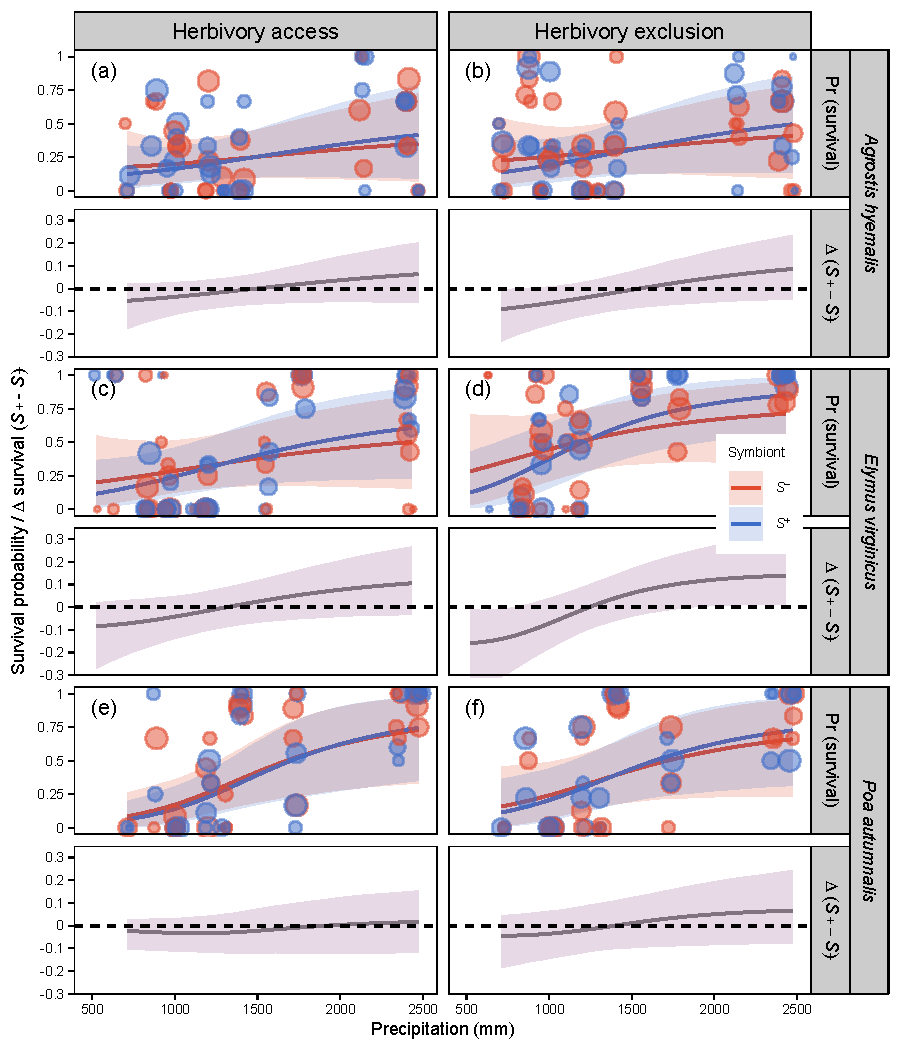
\includegraphics[width=1\textwidth]{../Figure/PrSurvival_diff.pdf}
\caption{Predicted survival rate (top panels) and endophyte effect (\(\Delta = \mathrm{E^+ - E^-}\), bottom panels) across precipitation gradients. 
Lines show posterior means for E\(^+\) (blue) and E\(^-\) (red), with shading indicating 90\% credible intervals. 
Points represent mean observed survival per plot,  jittered  for visualization.  
The dashed line at \(\Delta = 0\) indicates no endophyte effect. 
Panels are organized by species and herbivory treatment (Fenced, Unfenced).}
\label{fig:Surv}
\end{figure}

\begin{figure}[H]
\centering
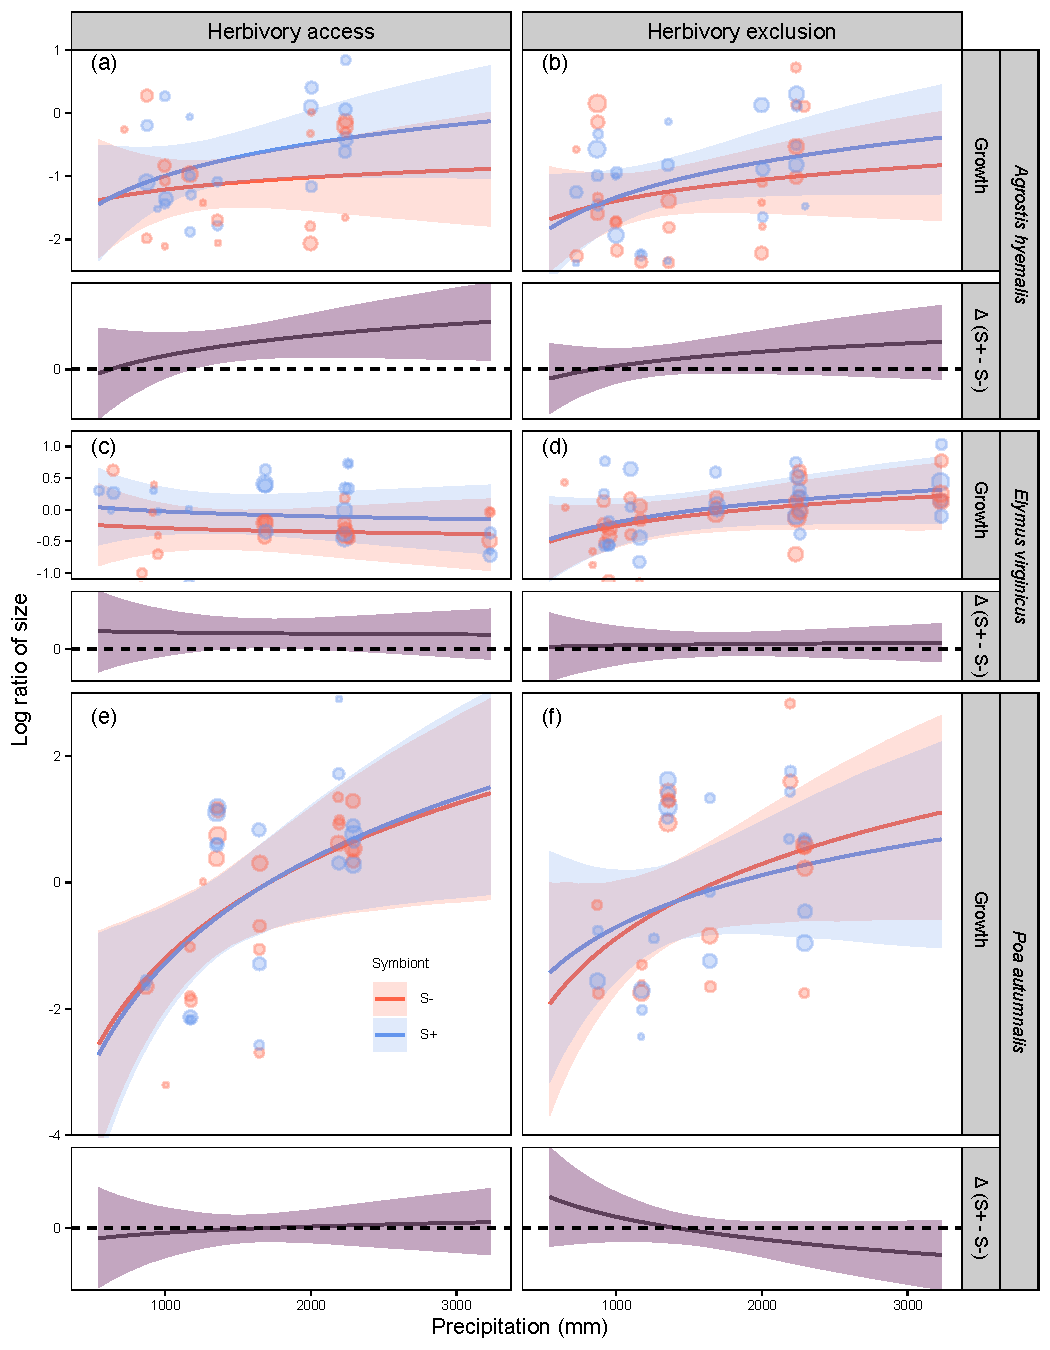
\includegraphics[width=0.8\textwidth]{../Figure/Growth_diff.pdf}
\caption{Predicted relative growth from year to the next year (top panels) and endophyte effect (\(\Delta = \mathrm{E^+ - E^-}\), bottom panels) across precipitation gradients. 
Lines show posterior means for E\(^+\) (blue) and E\(^-\) (red), with shading indicating 90\% credible intervals. 
Points represent mean observed growth per plot,  jittered  for visualization.  
The dashed line at \(\Delta = 0\) indicates no endophyte effect. 
Panels are organized by species and herbivory treatment (Fenced, Unfenced).}
\label{fig:growth}
\end{figure}

\begin{figure}[H]
\centering
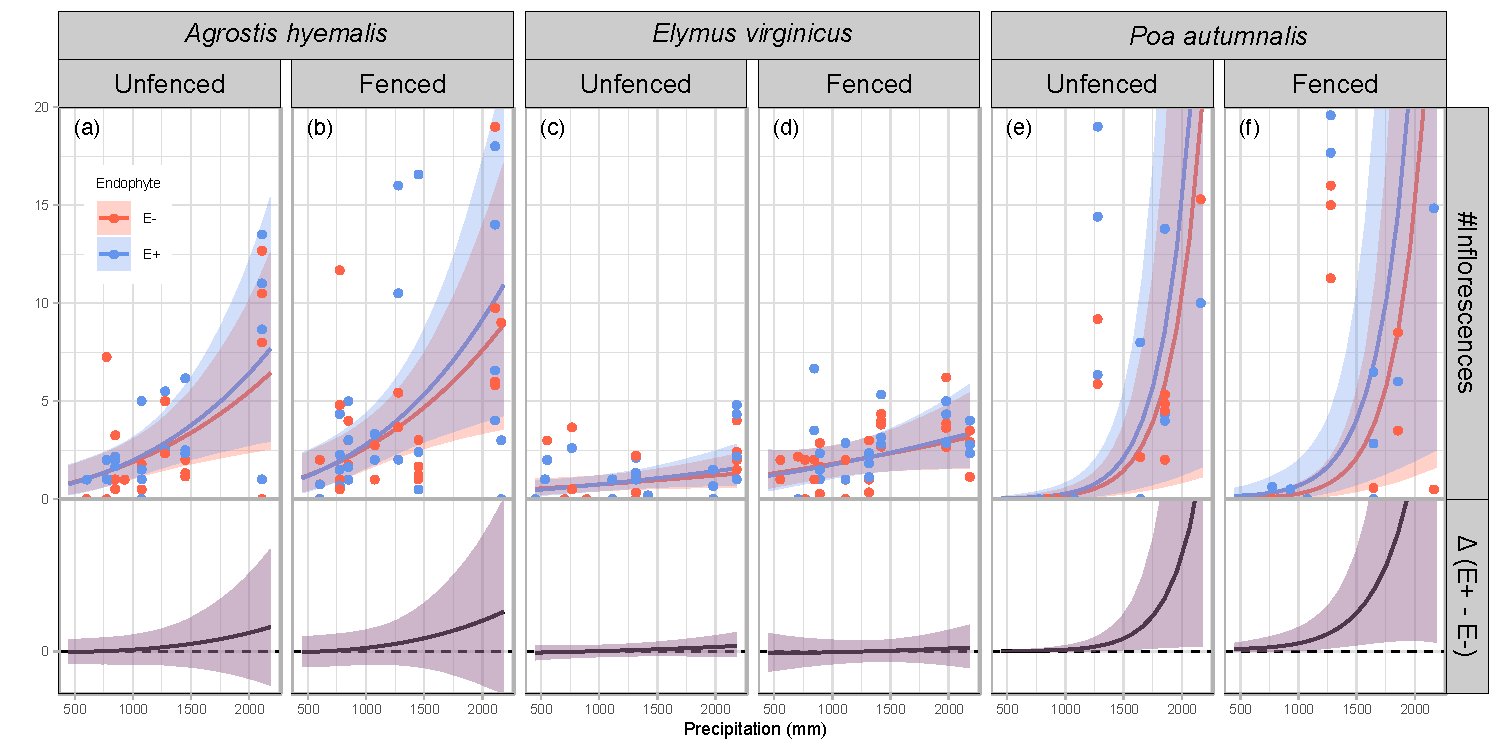
\includegraphics[width=1\textwidth]{../Figure/Flowering_diff_v.pdf}
\caption{
%Effects of precipitation, endophyte presence, and herbivory on flowering output (number of inflorescences) across three cool-season grass species. 
Predicted number of inflorescences (upper panels) and the difference between endophyte-infected (E$^+$) and endophyte-free (E$^-$) plants ($\Delta$(E$^+$--E$^-$), lower panels) are shown across a gradient of precipitation.
%for \textit{Agrostis hyemalis}, \textit{Elymus virginicus}, and \textit{Poa autumnalis}. 
Shaded areas represent 90\% credible intervals. 
Points indicate observed means,jittered  for visualization. 
Panels are grouped by species and herbivory treatment (unfenced = with herbivory; fenced = herbivory excluded).}
\label{fig:flowering}
\end{figure}


\begin{figure}[H]
\centering
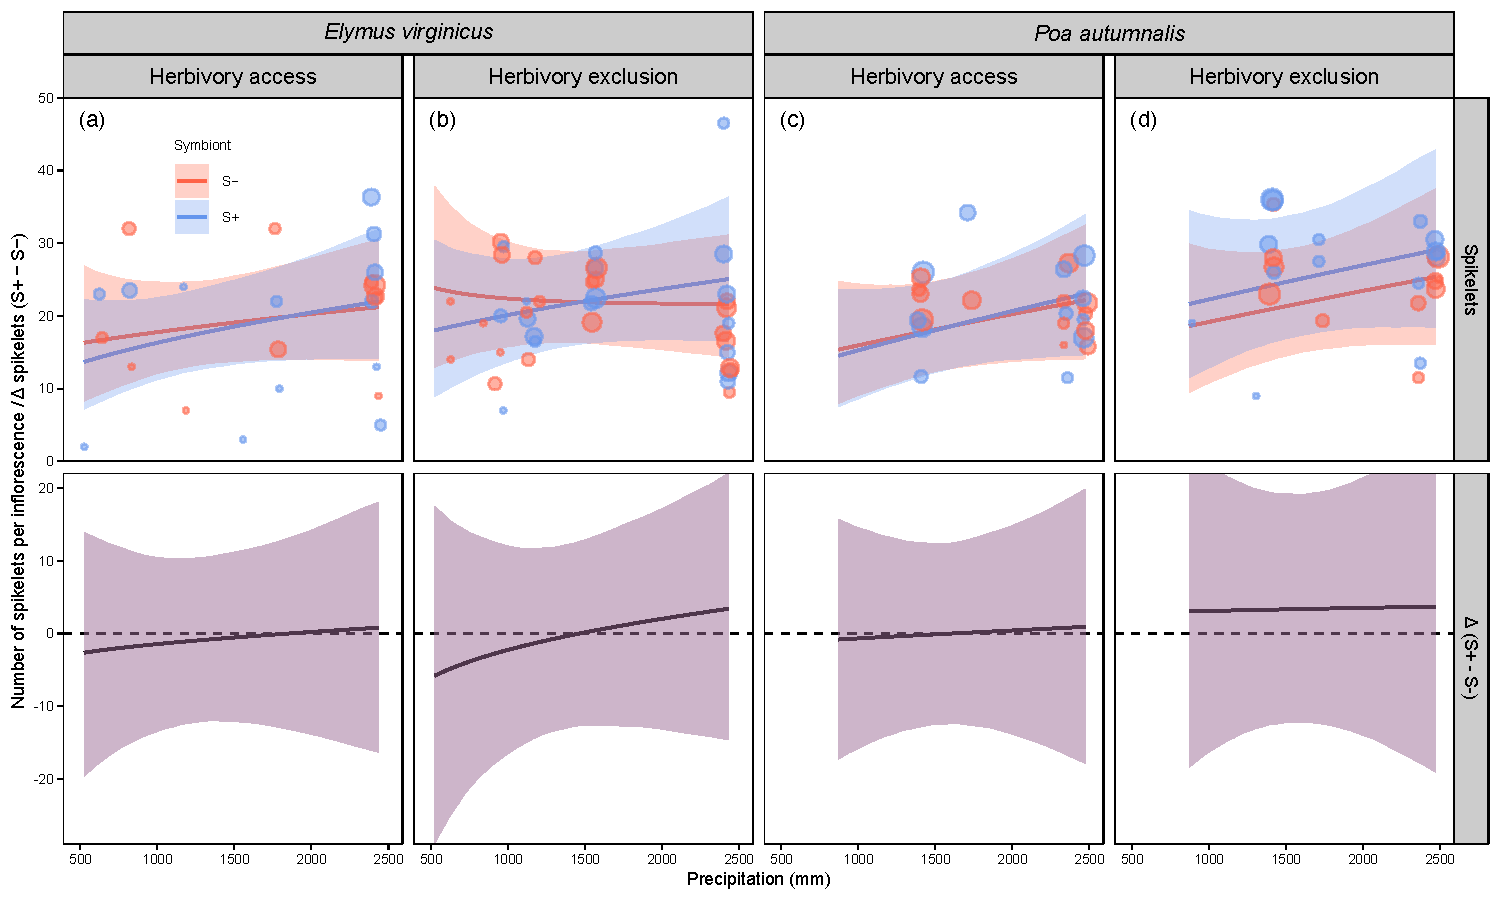
\includegraphics[width=0.8\textwidth]{../Figure/Spikelet_diff.pdf}
\caption{Predicted number of spikelets (upper panels) and endophyte effect (\(\Delta = \mathrm{E^+ - E^-}\), bottom panels) across precipitation gradients. 
Lines show posterior means for E\(^+\) (blue) and E\(^-\) (red), with shading indicating 90\% credible intervals. 
Points represent mean observed spikelets per plot, slightly jittered for visualization. 
Spikelets were measured for only two species (see Methods for details).  
The dashed line at \(\Delta = 0\) indicates no endophyte effect. 
Panels are organized by species and herbivory treatment (Fenced, Unfenced).}
\label{fig:spikelet}
\end{figure}

\subsection*{Abiotic factors as the primary drivers of fitness components across the stress gradient}
Across all vital rates (survival, growth, inflorescence, and spikelet production), models that included only abiotic predictors consistently provided the best fits, measured by expected log predictive density (ELPD; higher values indicate better predictive accuracy; Figure~\ref{fig:bestdriver}).  
Uncertainty estimates showed that in some cases the advantage of abiotic-only models over those that also included biotic predictors was small. 
For example, for survival, the abiotic-only model outperformed the abiotic and biotic model only slightly 
($\Delta \mathrm{ELPD} = -2.1$, SE = 3.7), suggesting that adding biotic predictors contributed little additional explanatory power.  
By contrast, models based only on biotic factors performed much worse (e.g., survival: $\Delta \mathrm{ELPD} = -5.2$, SE = 2.0).  
Taken together, these results suggest that the demography of \textit{Agrostis hyemalis}, \textit{Elymus virginicus}, and \textit{Poa autumnalis} 
is shaped primarily by abiotic stress related to precipitation, while \tom{biotic interactions (herbivory and endophyte presence) play a secondary role. }{Following my comments above, I think this analysis would be better focused if all models included endophyte, and we are comparing endo*precip against endo*herb against endo*precip*herb. I don't think it is particularly meaningful that abiotic stress was stronger than the effect of endophytes -- that does not surprise me and in some sense is not the point of the experiment. We really want to know what are the factors that make this symbiosis more mutualistic or more parasitic.}
\tom{This pattern aligns with the stress gradient hypothesis, which predicts that abiotic factors dominate in stressful environments, whereas biotic interactions gain importance under more benign conditions.}{I actually don't think it aligns with the SGH for two reasons. First, this analysis is currently saying that precip is more important for demography than biotic interactions. That is not the SGH. The SGH is about whether *species interactions* become more positive under stress. The second reason is that you found the opposite: the symbiosis became *less positive* under stress!}
\tom{}{I really like this analysis! This is another place where I think readers will need more guidance about what the alternative expectations might be, so that they could interpret this figure appropriately. If these points are averages why does abiotic have no error bars? Is it weird that the abiotic-biotic error bars exceed zero?}

%\begin{figure}[H]
%    \centering
%    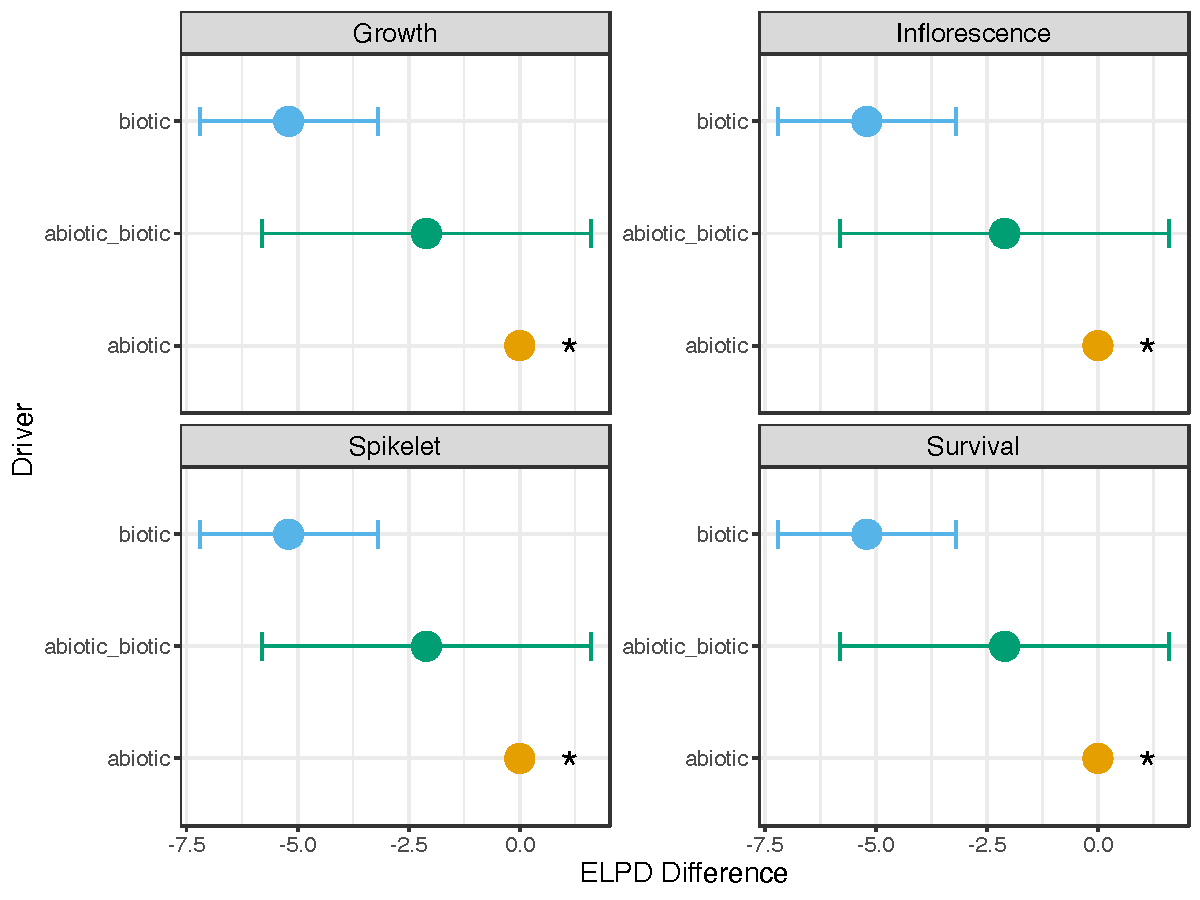
\includegraphics[width=1\textwidth]{../Figure/bestdriver.pdf}
%    \caption{Model comparison across vital rates (survival, growth, flowering, spikelet production) using expected log predictive density (ELPD) differences. 
%    ELPD measures a model's ability to predict new data, with higher values indicating better predictive performance. Differences in ELPD relative to the best-supported model (abiotic-only) show which models perform better or worse. 
%    Circles indicate the ELPD of each model, error bars represent the standard error of the differences (SE), and stars mark the model with the highest ELPD. 
%%    Abiotic-only models consistently performed best, while differences between abiotic-only and abiotic+biotic models were generally small relative to SE, suggesting marginal improvement from adding biotic predictors. 
%%    Biotic-only models were consistently inferior, with $\Delta$ELPD larger than the SE, indicating clear underperformance. This comparison highlights that abiotic variation primarily drives the demography of \textit{Agrostis hyemalis}, \textit{Elymus virginicus}, and \textit{Poa autumnalis}.
%     }
%    \label{fig:bestdriver}
%\end{figure}
%


\section*{Acknowledgements}
This research was supported by National Science Foundation Division of Environmental Biology awards.



\newpage
\bibliographystyle{apalike}
\bibliography{References}
%--------------------------------------------------------------------
\newpage
\clearpage 
\setcounter{equation}{0}
\setcounter{figure}{0}
\setcounter{section}{0}
\setcounter{table}{0}
\renewcommand{\theequation}{S.\arabic{equation}}
\renewcommand{\thetable}{S-\arabic{table}}
\renewcommand{\thefigure}{S-\arabic{figure}}
\renewcommand{\thesection}{S.\arabic{section}}

\centerline{\Large{\textbf{Supporting Information}}}
\subsection{Candidate models for abiotic and biotic drivers of cool-grass species} \label{sec:models}
\begin{enumerate}
    \item \textbf{Abiotic model:} includes precipitation ($P$) and its quadratic term ($P^2$) as predictors, along with endophyte status ($\text{endo}$) and its interactions with climate. Species-specific effects borrow strength across species:
    \begin{align*}
    \mu_i &= \beta_0[\text{Sp}_i] + \beta_{\text{endo}}[\text{Sp}_i]\,endo_i + \beta_P[\text{Sp}_i] P_i + \beta_{P^2}[\text{Sp}_i] P_i^2 
            + \beta_{\text{endo}\times P}[\text{Sp}_i]\,endo_i P_i 
            + \beta_{\text{endo}\times P^2}[\text{Sp}_i]\,endo_i P_i^2 \\
    &\quad + \phi_{\text{site}[i],\text{Sp}_i} + \omega_{\text{source}[i],\text{Sp}_i} + \rho_{\text{plot}[i],\text{Sp}_i}
    \end{align*}

    \item \textbf{Biotic model:} includes endophyte status ($\text{endo}$), herbivory ($\text{herb}$), and their interaction, with species-specific effects:
    \begin{align*}
    \mu_i &= \beta_0[\text{Sp}_i] + \beta_{\text{endo}}[\text{Sp}_i]\,endo_i + \beta_{\text{herb}}[\text{Sp}_i]\,herb_i 
            + \beta_{\text{endo}\times \text{herb}}[\text{Sp}_i]\,endo_i\,herb_i \\
    &\quad + \phi_{\text{site}[i],\text{Sp}_i} + \omega_{\text{source}[i],\text{Sp}_i} + \rho_{\text{plot}[i],\text{Sp}_i}
    \end{align*}

    \item \textbf{Full model:} combines abiotic and biotic predictors, including all relevant interactions up to the three-way interaction between endophyte, herbivory, and precipitation, with species-varying coefficients:
    \begin{align*}
    \mu_i &= \beta_0[\text{Sp}_i] + \beta_P[\text{Sp}_i] P_i + \beta_{P^2}[\text{Sp}_i] P_i^2 + \beta_{\text{endo}}[\text{Sp}_i]\,endo_i + \beta_{\text{herb}}[\text{Sp}_i]\,herb_i \\
    &\quad + \beta_{\text{endo}\times P}[\text{Sp}_i]\,endo_i P_i 
          + \beta_{\text{endo}\times P^2}[\text{Sp}_i]\,endo_i P_i^2
          + \beta_{\text{herb}\times P}[\text{Sp}_i]\,herb_i P_i 
          + \beta_{\text{herb}\times \text{endo}}[\text{Sp}_i]\,herb_i\,endo_i \\
    &\quad + \beta_{\text{endo}\times \text{herb} \times P}[\text{Sp}_i]\,endo_i\,herb_i\,P_i
          + \phi_{\text{site}[i],\text{Sp}_i} + \omega_{\text{source}[i],\text{Sp}_i} + \rho_{\text{plot}[i],\text{Sp}_i}
    \end{align*}
\end{enumerate}
In these models, the $\beta$ coefficients represent species-specific effects. 
The intercept $\beta_0[\text{Sp}_i]$ corresponds to the baseline value of the vital rate for species $\text{Sp}_i$ in the absence of predictors. $\beta_{\text{endo}}[\text{Sp}_i]$ and $\beta_{\text{herb}}[\text{Sp}_i]$ describe the effects of endophyte presence and herbivory, respectively, for species $\text{Sp}_i$. 
The linear and quadratic effects of precipitation are captured by $\beta_P[\text{Sp}_i]$ and $\beta_{P^2}[\text{Sp}_i]$, while interactions between endophyte and precipitation are represented by $\beta_{\text{endo}\times P}[\text{Sp}_i]$ and $\beta_{\text{endo}\times P^2}[\text{Sp}_i]$. 
The interaction between endophyte and herbivory is given by $\beta_{\text{endo}\times \text{herb}}[\text{Sp}_i]$, the interaction between herbivory and precipitation by $\beta_{\text{herb}\times P}[\text{Sp}_i]$, and the three-way interaction among endophyte, herbivory, and precipitation by $\beta_{\text{endo}\times \text{herb} \times P}[\text{Sp}_i]$. All $\beta$ coefficients are modeled hierarchically across species, allowing information to be shared while capturing species-specific responses.
All models included a hierarchical random effects structure accounting for site-year, source population, and plot variation, with species-specific random effects $\phi_{\text{site}[i],\text{Sp}_i} \sim \mathcal{N}(0, \sigma_{\text{site}})$, $\omega_{\text{source}[i],\text{Sp}_i} \sim \mathcal{N}(0, \sigma_{\text{source}})$, and $\rho_{\text{plot}[i],\text{Sp}_i} \sim \mathcal{N}(0, \sigma_{\text{plot}})$.

\section {Supporting Tables}
\begin{table}[ht]
\centering
\caption{Geographic coordinates and brief descriptions of source populations for \textit{Agrostis hyemalis} (AGHY), \textit{Elymus virginicus} (ELVI), and \textit{Poa autumnalis} (POAU).}
\label{tab:source_pop}
\begin{tabular}{lllll}
\toprule
\textbf{Species} & \textbf{Population} & \textbf{Latitude} & \textbf{Longitude} & \textbf{Description} \\
\midrule
AGHY & SJC  & 30.771969 & -95.200620 & Ecolab property \\
AGHY & COHR & 29.672833 & -96.567517 & Columbus, TX herbarium record \\
AGHY & LPEF & 30.085383 & -97.172508 & Lost Pines \\
POAU & LA7  & 30.849660 & -93.276772 & DeRidder, LA \\
POAU & LA1  & 32.568125 & -93.932976 & Jean Lafitte National Historical Park and Preserve \\
POAU & LA2  & 31.183040 & -92.616969 & Jean Lafitte National Historical Park and Preserve \\
POAU & SFAEF & 31.492158 & -94.772200 & Stephen F. Austin Experimental Forest, TX \\
POAU & WB   & 30.399346 & -95.150026 & Sam Houston National Forest \\
ELVI & HUNT & 30.741797 & -95.474508 & Sam Houston State University Field Station \\
ELVI & SHS  & 30.741797 & -95.474508 & Sam Houston State University Field Station \\
ELVI & RL5  & 30.471717 & -99.783803 & Texas Tech University, Junction \\
ELVI & PALM & 29.591623 & -97.584781 & Palmetto State Park, TX \\
ELVI & JLP  & 29.785105 & -90.114933 & Jean Lafitte Park, outside of New Orleans \\
\bottomrule
\end{tabular}
\end{table}

\begin{table}[ht]
\centering
\caption{Common garden and field experiment sites used for reciprocal transplant and environmental manipulation studies.}
\label{tab:exp_sites}
\begin{tabular}{llrr}
\hline
\textbf{Site} & \textbf{Code} & \textbf{Latitude} & \textbf{Longitude} \\
\hline
University of Louisiana Ecology Center & LAF & 30.304773 & -92.012401 \\
Center for Biological Field Studies & HUN & 30.742815 & -95.476881 \\
TAMU Ecology and Natural Resource Teaching Area & COL & 30.569302 & -96.366324 \\
UT Stengl Lost Pines Field Station & BAS & 30.092343 & -97.172442 \\
1335 Medina Hwy, Kerrville, TX & KER & 30.028437 & -99.142888 \\
Brackenridge Field Laboratory & BFL & 30.284866 & -97.780675 \\
TAMU Sonora Station & SON & 30.273467 & -100.561463 \\
\hline
\end{tabular}
\end{table}

\begin{landscape}
\begin{table}[ht]
\centering
\small
\caption{Posterior summaries of $\Delta$ (E$^{+}$ $-$ E$^{-}$) at precipitation quantiles for each species and herbivore exclusion treatment. Median, 90\% credible interval, and posterior probability that $\Delta > 0$ are shown. Herbivore exclusion: Fenced = herbivores excluded, Unfenced = herbivores had access.}
\label{tab:delta_summary_surv}
\begin{tabular}{llrrrrr}
\hline
Species & Herbivore exclusion & Precipitation (mm) & P($\Delta>0$) & Median & Lower 90\% & Upper 90\% \\
\hline
\textit{Agrostis hyemalis} & Unfenced & 765.76 & 0.40 & -0.007 & -0.092 & 0.063 \\
\textit{Agrostis hyemalis} & Unfenced & 848.28 & 0.44 & -0.005 & -0.082 & 0.064 \\
\textit{Agrostis hyemalis} & Unfenced & 1113.25 & 0.55 & 0.004  & -0.065 & 0.076 \\
\textit{Agrostis hyemalis} & Unfenced & 1644.36 & 0.69 & 0.021  & -0.063 & 0.129 \\
\textit{Agrostis hyemalis} & Unfenced & 2163.28 & 0.74 & 0.033  & -0.067 & 0.178 \\
\textit{Agrostis hyemalis} & Fenced   & 765.76 & 0.12 & -0.042 & -0.149 & 0.020 \\
\textit{Agrostis hyemalis} & Fenced   & 848.28 & 0.14 & -0.038 & -0.135 & 0.022 \\
\textit{Agrostis hyemalis} & Fenced   & 1113.25 & 0.25 & -0.025 & -0.107 & 0.039 \\
\textit{Agrostis hyemalis} & Fenced   & 1644.36 & 0.53 & 0.004  & -0.097 & 0.106 \\
\textit{Agrostis hyemalis} & Fenced   & 2163.28 & 0.66 & 0.025  & -0.098 & 0.173 \\
\textit{Elymus virginicus} & Unfenced & 765.76 & 0.43 & -0.013 & -0.138 & 0.109 \\
\textit{Elymus virginicus} & Unfenced & 848.28 & 0.48 & -0.004 & -0.127 & 0.117 \\
\textit{Elymus virginicus} & Unfenced & 1113.25 & 0.63 & 0.023  & -0.098 & 0.147 \\
\textit{Elymus virginicus} & Unfenced & 1644.36 & 0.80 & 0.067  & -0.068 & 0.208 \\
\textit{Elymus virginicus} & Unfenced & 2163.28 & 0.85 & 0.084  & -0.054 & 0.251 \\
\textit{Elymus virginicus} & Fenced   & 765.76 & 0.18 & -0.074 & -0.215 & 0.060 \\
\textit{Elymus virginicus} & Fenced   & 848.28 & 0.24 & -0.054 & -0.182 & 0.070 \\
\textit{Elymus virginicus} & Fenced   & 1113.25 & 0.50 & 0.001  & -0.109 & 0.109 \\
\textit{Elymus virginicus} & Fenced   & 1644.36 & 0.82 & 0.056  & -0.045 & 0.186 \\
\textit{Elymus virginicus} & Fenced   & 2163.28 & 0.89 & 0.068  & -0.026 & 0.237 \\
\textit{Poa autumnalis}    & Unfenced & 765.76 & 0.21 & -0.012 & -0.095 & 0.020 \\
\textit{Poa autumnalis}    & Unfenced & 848.28 & 0.19 & -0.018 & -0.115 & 0.024 \\
\textit{Poa autumnalis}    & Unfenced & 1113.25 & 0.17 & -0.050 & -0.175 & 0.041 \\
\textit{Poa autumnalis}    & Unfenced & 1644.36 & 0.20 & -0.052 & -0.191 & 0.053 \\
\textit{Poa autumnalis}    & Unfenced & 2163.28 & 0.25 & -0.014 & -0.142 & 0.037 \\
\textit{Poa autumnalis}    & Fenced   & 765.76 & 0.64 & 0.005  & -0.039 & 0.077 \\
\textit{Poa autumnalis}    & Fenced   & 848.28 & 0.65 & 0.008  & -0.048 & 0.092 \\
\textit{Poa autumnalis}    & Fenced   & 1113.25 & 0.69 & 0.025  & -0.074 & 0.143 \\
\textit{Poa autumnalis}    & Fenced   & 1644.36 & 0.67 & 0.027  & -0.092 & 0.166 \\
\textit{Poa autumnalis}    & Fenced   & 2163.28 & 0.64 & 0.007  & -0.071 & 0.124 \\
\hline
\end{tabular}
\end{table}
\end{landscape}

\begin{landscape}
\begin{table}[ht]
\centering
\small
\caption{Posterior summaries of $\Delta$ (E$^{+}$ $-$ E$^{-}$) for growth at precipitation quantiles for each species and herbivore exclusion treatment. Median, 90\% credible interval, and posterior probability that $\Delta > 0$ are shown. Herbivore exclusion: Fenced = herbivores excluded, Unfenced = herbivores had access.}
\label{tab:delta_summary_grow}
\begin{tabular}{llrrrrr}
\hline
Species & Herbivore exclusion & Precipitation (mm) & Median & Lower 90\% & Upper 90\% & P($\Delta>0$) \\
\hline
\textit{Agrostis hyemalis} & Unfenced & 773.91  & 0.3972  & 0.0415  & 0.7575  & 0.9653 \\
\textit{Agrostis hyemalis} & Unfenced & 1075.09 & 0.4090  & 0.1241  & 0.6904  & 0.9908 \\
\textit{Agrostis hyemalis} & Unfenced & 1316.25 & 0.4135  & 0.1361  & 0.6882  & 0.9924 \\
\textit{Agrostis hyemalis} & Unfenced & 1979.35 & 0.4246  & 0.0621  & 0.7877  & 0.9734 \\
\textit{Agrostis hyemalis} & Unfenced & 2163.28 & 0.4259  & 0.0343  & 0.8226  & 0.9636 \\
\textit{Agrostis hyemalis} & Fenced   & 773.91  & 0.0914  & -0.2214 & 0.3987  & 0.6861 \\
\textit{Agrostis hyemalis} & Fenced   & 1075.09 & 0.1362  & -0.1095 & 0.3711  & 0.8163 \\
\textit{Agrostis hyemalis} & Fenced   & 1316.25 & 0.1636  & -0.0892 & 0.4085  & 0.8550 \\
\textit{Agrostis hyemalis} & Fenced   & 1979.35 & 0.2207  & -0.1445 & 0.5769  & 0.8374 \\
\textit{Agrostis hyemalis} & Fenced   & 2163.28 & 0.2335  & -0.1646 & 0.6227  & 0.8300 \\
\textit{Elymus virginicus} & Unfenced & 773.91  & 0.2673  & -0.0977 & 0.6250  & 0.8831 \\
\textit{Elymus virginicus} & Unfenced & 1075.09 & 0.2641  & -0.0129 & 0.5294  & 0.9428 \\
\textit{Elymus virginicus} & Unfenced & 1316.25 & 0.2597  & 0.0157  & 0.5034  & 0.9583 \\
\textit{Elymus virginicus} & Unfenced & 1979.35 & 0.2535  & -0.0271 & 0.5406  & 0.9298 \\
\textit{Elymus virginicus} & Unfenced & 2163.28 & 0.2521  & -0.0492 & 0.5591  & 0.9155 \\
\textit{Elymus virginicus} & Fenced   & 773.91  & 0.0386  & -0.2904 & 0.3763  & 0.5755 \\
\textit{Elymus virginicus} & Fenced   & 1075.09 & 0.0659  & -0.1541 & 0.2925  & 0.6887 \\
\textit{Elymus virginicus} & Fenced   & 1316.25 & 0.0824  & -0.1096 & 0.2760  & 0.7598 \\
\textit{Elymus virginicus} & Fenced   & 1979.35 & 0.1139  & -0.1361 & 0.3706  & 0.7695 \\
\textit{Elymus virginicus} & Fenced   & 2163.28 & 0.1208  & -0.1581 & 0.4035  & 0.7571 \\
\textit{Poa autumnalis}    & Unfenced & 773.91  & -0.1283 & -0.5443 & 0.2965  & 0.3020 \\
\textit{Poa autumnalis}    & Unfenced & 1075.09 & -0.0666 & -0.3546 & 0.2256  & 0.3537 \\
\textit{Poa autumnalis}    & Unfenced & 1316.25 & -0.0270 & -0.2636 & 0.2113  & 0.4236 \\
\textit{Poa autumnalis}    & Unfenced & 1979.35 & 0.0519  & -0.2103 & 0.3156  & 0.6258 \\
\textit{Poa autumnalis}    & Unfenced & 2163.28 & 0.0688  & -0.2201 & 0.3586  & 0.6500 \\
\textit{Poa autumnalis}    & Fenced   & 773.91  & 0.3338  & -0.0740 & 0.7568  & 0.9119 \\
\textit{Poa autumnalis}    & Fenced   & 1075.09 & 0.1388  & -0.1364 & 0.4275  & 0.7897 \\
\textit{Poa autumnalis}    & Fenced   & 1316.25 & 0.0181  & -0.2156 & 0.2530  & 0.5503 \\
\textit{Poa autumnalis}    & Fenced   & 1979.35 & -0.2281 & -0.5148 & 0.0604  & 0.0963 \\
\textit{Poa autumnalis}    & Fenced   & 2163.28 & -0.2822 & -0.6016 & 0.0377  & 0.0727 \\
\hline
\end{tabular}
\end{table}
\end{landscape}

\begin{landscape}
\begin{table}[htbp]
\centering
\caption{Posterior summaries of $\Delta$ (E$^{+}$ $-$ E$^{-}$) for \textbf{flowering output} at precipitation quantiles for each species and herbivore exclusion treatment. Median, 90\% credible interval, and posterior probability that $\Delta > 0$ are shown. Herbivore exclusion: Fenced = herbivores excluded, Unfenced = herbivores had access.}
\label{tab:delta_summary_flow}
\begin{tabular}{llrrrrr}
\hline
Species & Herbivore exclusion & Precipitation (mm) & Median & Lower 90\% & Upper 90\% & P($\Delta>0$) \\
\hline
\textit{Agrostis hyemalis} & Unfenced & 773.91  & 0.0014  & -0.1102  & 0.1129  & 0.5090 \\
\textit{Agrostis hyemalis} & Unfenced & 1075.09 & 0.0118  & -0.0654  & 0.0910  & 0.5990 \\
\textit{Agrostis hyemalis} & Unfenced & 1316.25 & 0.0161  & -0.0473  & 0.0830  & 0.6653 \\
\textit{Agrostis hyemalis} & Unfenced & 1979.35 & 0.0185  & -0.0350  & 0.0785  & 0.7277 \\
\textit{Agrostis hyemalis} & Unfenced & 2163.28 & 0.0178  & -0.0350  & 0.0782  & 0.7303 \\
\textit{Agrostis hyemalis} & Fenced   & 773.91  & 0.0042  & -0.0883  & 0.0937  & 0.5313 \\
\textit{Agrostis hyemalis} & Fenced   & 1075.09 & 0.0139  & -0.0429  & 0.0716  & 0.6579 \\
\textit{Agrostis hyemalis} & Fenced   & 1316.25 & 0.0171  & -0.0299  & 0.0655  & 0.7329 \\
\textit{Agrostis hyemalis} & Fenced   & 1979.35 & 0.0172  & -0.0246  & 0.0649  & 0.7679 \\
\textit{Agrostis hyemalis} & Fenced   & 2163.28 & 0.0164  & -0.0247  & 0.0650  & 0.7666 \\
\textit{Elymus virginicus} & Unfenced & 773.91  & -0.0101 & -0.1184  & 0.0989  & 0.4403 \\
\textit{Elymus virginicus} & Unfenced & 1075.09 & 0.0067  & -0.0820  & 0.0965  & 0.5482 \\
\textit{Elymus virginicus} & Unfenced & 1316.25 & 0.0178  & -0.0638  & 0.1018  & 0.6353 \\
\textit{Elymus virginicus} & Unfenced & 1979.35 & 0.0394  & -0.0490  & 0.1320  & 0.7626 \\
\textit{Elymus virginicus} & Unfenced & 2163.28 & 0.0436  & -0.0501  & 0.1403  & 0.7764 \\
\textit{Elymus virginicus} & Fenced   & 773.91  & -0.0141 & -0.1245  & 0.0934  & 0.4158 \\
\textit{Elymus virginicus} & Fenced   & 1075.09 & -0.0057 & -0.0768  & 0.0631  & 0.4470 \\
\textit{Elymus virginicus} & Fenced   & 1316.25 & -0.0005 & -0.0548  & 0.0529  & 0.4931 \\
\textit{Elymus virginicus} & Fenced   & 1979.35 & 0.0082  & -0.0469  & 0.0625  & 0.5966 \\
\textit{Elymus virginicus} & Fenced   & 2163.28 & 0.0096  & -0.0505  & 0.0693  & 0.6075 \\
\textit{Poa autumnalis}    & Unfenced & 773.91  & 0.0105  & -0.0073  & 0.0892  & 0.8576 \\
\textit{Poa autumnalis}    & Unfenced & 1075.09 & 0.0457  & -0.0011  & 0.1332  & 0.9457 \\
\textit{Poa autumnalis}    & Unfenced & 1316.25 & 0.0758  & 0.0143   & 0.1466  & 0.9819 \\
\textit{Poa autumnalis}    & Unfenced & 1979.35 & 0.0391  & 0.0058   & 0.1151  & 0.9907 \\
\textit{Poa autumnalis}    & Unfenced & 2163.28 & 0.0257  & 0.0024   & 0.1049  & 0.9845 \\
\textit{Poa autumnalis}    & Fenced   & 773.91  & 0.0760  & 0.0099   & 0.2694  & 0.9978 \\
\textit{Poa autumnalis}    & Fenced   & 1075.09 & 0.1586  & 0.0552   & 0.2691  & 0.9998 \\
\textit{Poa autumnalis}    & Fenced   & 1316.25 & 0.1621  & 0.0831   & 0.2386  & 1.0000 \\
\textit{Poa autumnalis}    & Fenced   & 1979.35 & 0.0383  & 0.0063   & 0.1273  & 0.9977 \\
\textit{Poa autumnalis}    & Fenced   & 2163.28 & 0.0213  & 0.0020   & 0.1048  & 0.9869 \\
\hline
\end{tabular}
\end{table}
\end{landscape}

\begin{landscape}
\begin{table}[ht]
\centering
\small
\caption{Posterior summaries of $\Delta$ (E$^{+}$ $-$ E$^{-}$) at precipitation quantiles for each species and herbivore exclusion treatment. Median, 90\% credible interval, and posterior probability that $\Delta > 0$ are shown. Herbivore exclusion: Fenced = herbivores excluded, Unfenced = herbivores had access.}
\label{tab:delta_summary_spike}
\begin{tabular}{llrrrrr}
\hline
Species & Herbivore exclusion & Precipitation (mm) & Median & Lower 90\% & Upper 90\% & P($\Delta>0$) \\
\hline
\textit{Agrostis hyemalis} & Unfenced & 1035.41 & -0.00350 & -0.01449 & 0.00659 & 0.278 \\
\textit{Agrostis hyemalis} & Unfenced & 1276.99 & -0.00153 & -0.01034 & 0.00701 & 0.383 \\
\textit{Agrostis hyemalis} & Unfenced & 1644.36 & 0.00074  & -0.00703 & 0.00873 & 0.563 \\
\textit{Agrostis hyemalis} & Unfenced & 2163.28 & 0.00290  & -0.00518 & 0.01234 & 0.732 \\
\textit{Agrostis hyemalis} & Unfenced & 2182.71 & 0.00296  & -0.00516 & 0.01247 & 0.735 \\
\textit{Agrostis hyemalis} & Fenced   & 1035.41 & -0.00206 & -0.01010 & 0.00490 & 0.314 \\
\textit{Agrostis hyemalis} & Fenced   & 1276.99 & 0.00018  & -0.00511 & 0.00546 & 0.523 \\
\textit{Agrostis hyemalis} & Fenced   & 1644.36 & 0.00263  & -0.00173 & 0.00770 & 0.840 \\
\textit{Agrostis hyemalis} & Fenced   & 2163.28 & 0.00502  & -0.00065 & 0.01232 & 0.925 \\
\textit{Agrostis hyemalis} & Fenced   & 2182.71 & 0.00509  & -0.00065 & 0.01248 & 0.926 \\
\textit{Elymus virginicus} & Unfenced & 1035.41 & -0.00382 & -0.01785 & 0.00782 & 0.285 \\
\textit{Elymus virginicus} & Unfenced & 1276.99 & -0.00172 & -0.01012 & 0.00598 & 0.349 \\
\textit{Elymus virginicus} & Unfenced & 1644.36 & 0.00035  & -0.00487 & 0.00559 & 0.548 \\
\textit{Elymus virginicus} & Unfenced & 2163.28 & 0.00204  & -0.00356 & 0.00841 & 0.735 \\
\textit{Elymus virginicus} & Unfenced & 2182.71 & 0.00210  & -0.00357 & 0.00858 & 0.738 \\
\textit{Elymus virginicus} & Fenced   & 1035.41 & 0.00776  & -0.00107 & 0.02302 & 0.920 \\
\textit{Elymus virginicus} & Fenced   & 1276.99 & 0.00672  & 0.00065  & 0.01582 & 0.966 \\
\textit{Elymus virginicus} & Fenced   & 1644.36 & 0.00557  & 0.00114  & 0.01134 & 0.982 \\
\textit{Elymus virginicus} & Fenced   & 2163.28 & 0.00436  & -0.00070 & 0.01108 & 0.923 \\
\textit{Elymus virginicus} & Fenced   & 2182.71 & 0.00432  & -0.00077 & 0.01111 & 0.919 \\
\hline
\end{tabular}
\end{table}
\end{landscape}


%\begin{table}[H]
%\caption{Model comparison by vital rate using ELPD (Expected Log Pointwise Density) differences. The values in the \textbf{elpd\_diff} column represent the difference in the model's ELPD relative to the best model for each vital rate, with positive values indicating a worse model fit. The \textbf{se\_diff} column shows the standard error of the ELPD difference. Best models for each vital rate are bolded. Model selection is based on the ELPD difference and associated standard error, with smaller ELPD differences and lower standard errors indicating better model fit.}
%
\begin{table}[H]
\caption{Differences in expected log predictive density (ELPD) between models for each vital rate. The top model for each response (bold) has the highest ELPD. Standard errors of the differences are shown in the \texttt{se\_diff} column.}
\centering
\begin{tabular}{|l|l|r|r|}
\hline
\textbf{Vital rate} & \textbf{Model} & \textbf{elpd\_diff} & \textbf{se\_diff} \\
\hline
Survival   & \textbf{abiotic}       & \textbf{0.0}  & \textbf{0.0} \\
           & abiotic\_biotic        & -2.1          & 3.7          \\
           & biotic                 & -5.2          & 2.0          \\
\hline
Growth     & \textbf{abiotic}       & \textbf{0.0}  & \textbf{0.0} \\
           & abiotic\_biotic        & -2.1          & 3.7          \\
           & biotic                 & -5.2          & 2.0          \\
\hline
Inflorescence & \textbf{abiotic}     & \textbf{0.0}  & \textbf{0.0} \\
              & abiotic\_biotic      & -2.1          & 3.7          \\
              & biotic               & -5.2          & 2.0          \\
\hline
Spikelet   & \textbf{abiotic}       & \textbf{0.0}  & \textbf{0.0} \\
           & abiotic\_biotic        & -2.1          & 3.7          \\
           & biotic                 & -5.2          & 2.0          \\
\hline
\end{tabular}
\label{tab:elpd_vital_rates}
\end{table}
\clearpage  % forces the next figure to start on a new page




\section {Supporting Figures}

\begin{figure}[H]
		\centering
		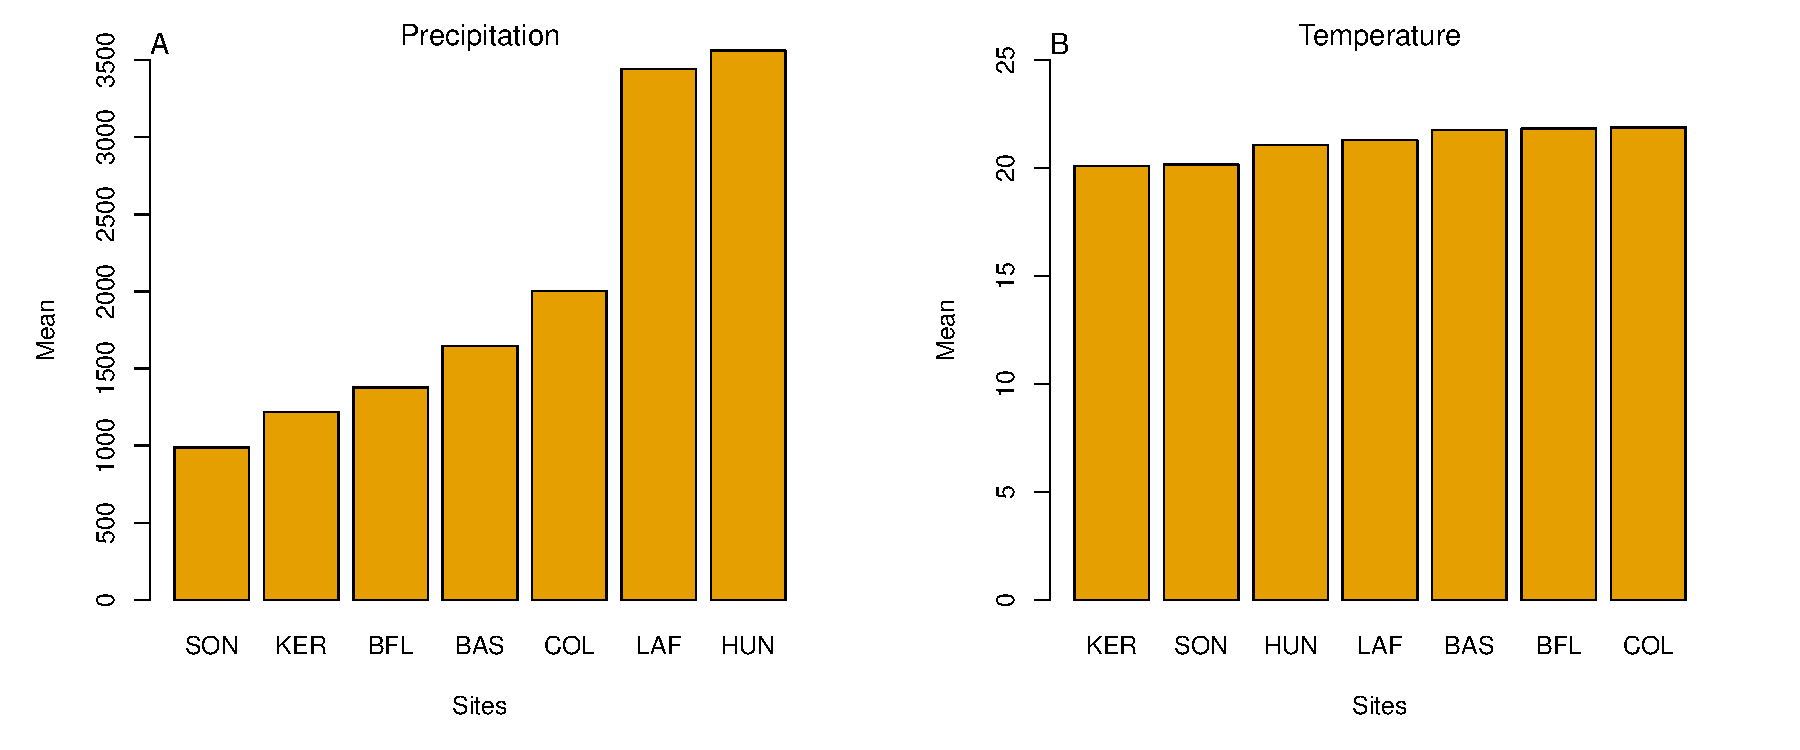
\includegraphics[width=1\linewidth]{../Figure/Climate_prism_2023_2025.pdf}
		\caption{Abiotic conditions across the seven study sites. 
		(A) Mean annual precipitation showing the pronounced east–west aridity gradient from mesic Louisiana to arid Texas. 
		(B) Mean annual temperature across sites, which does not differ much. 
		Panels highlight that precipitation, rather than temperature, constitutes the primary abiotic gradient in this system.}
		\label{Sup:temp}
\end{figure}
\clearpage  % forces the next figure to start on a new page

\begin{figure}[H]
\centering
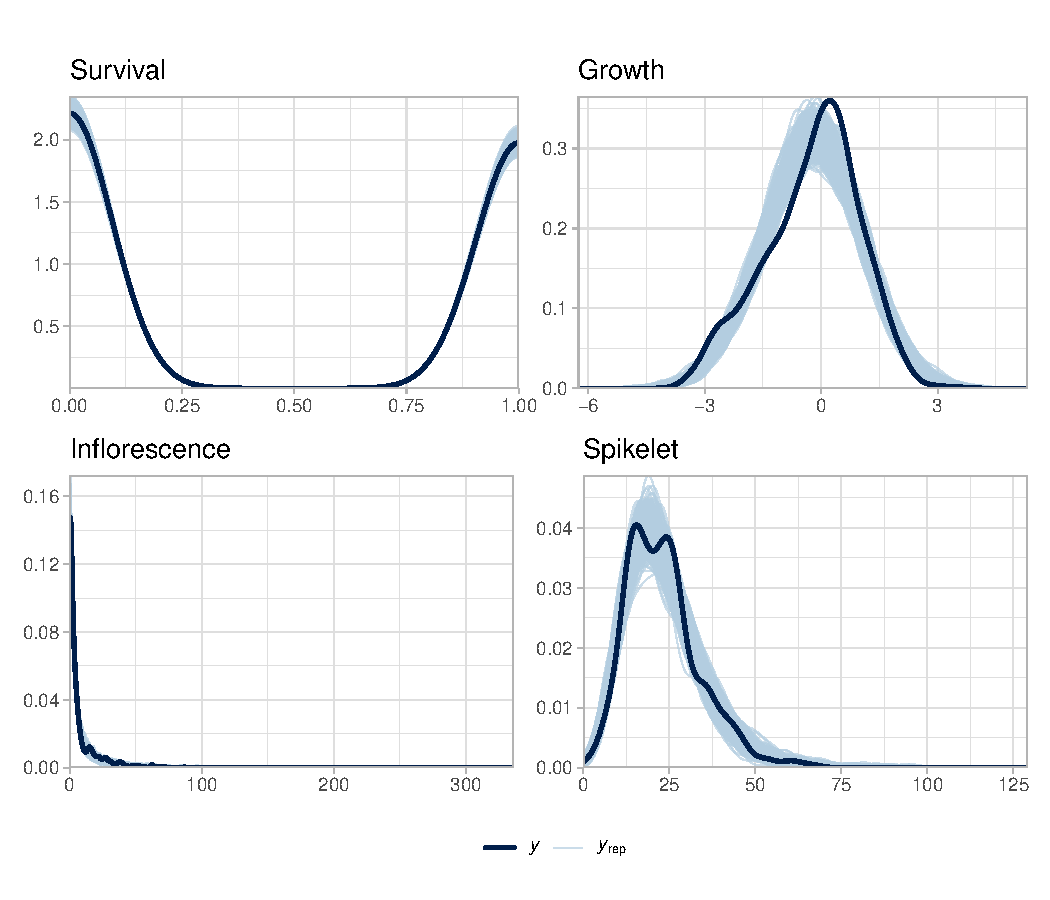
\includegraphics[width=1\textwidth]{../Figure/combined_ppc_plots.pdf}
\caption{
Posterior predictive checks for the full demographic model. 
Dark blue lines show observed data ($y$), and light blue lines show replicated datasets generated from posterior predictions ($y_{\text{rep}}$). 
The strong overlap across survival, growth, flowering, and spikelet production indicates adequate model fit for all vital rates.
}
\label{sup:ppc_vital}
\end{figure}

\begin{figure}[H]
		\centering
		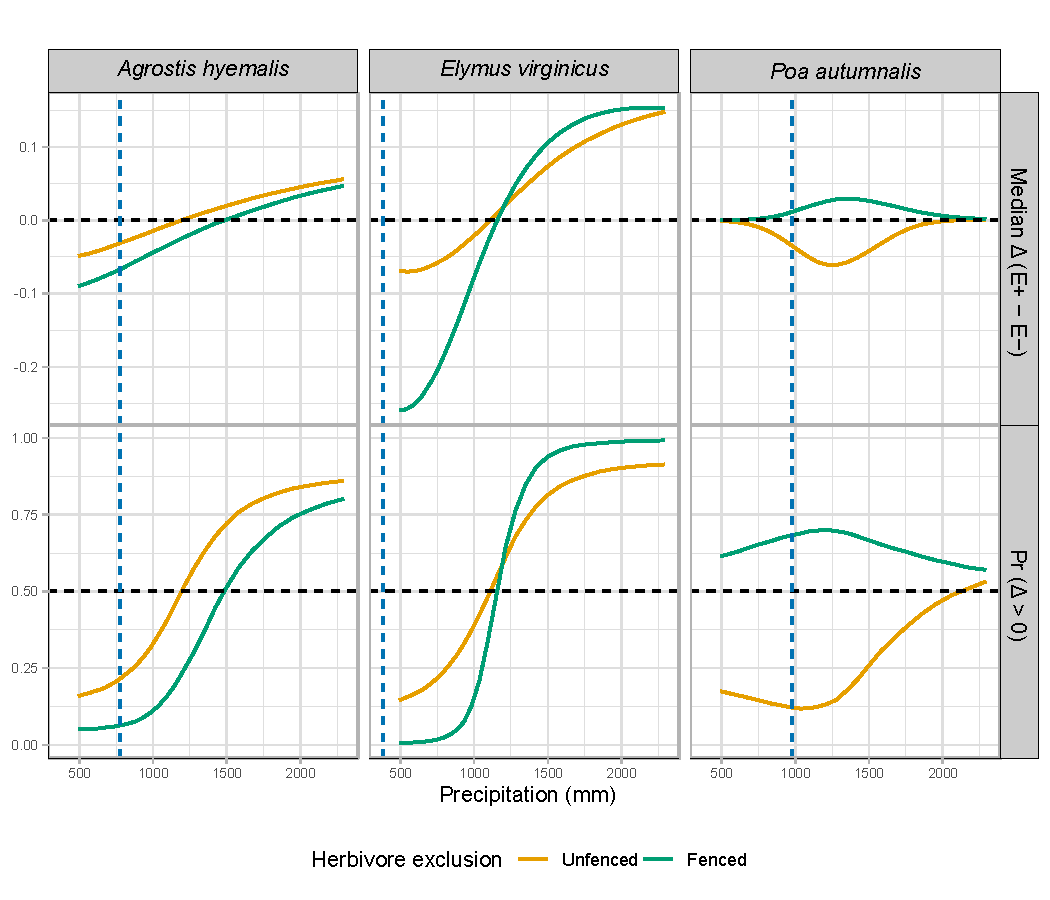
\includegraphics[width=1\linewidth]{../Figure/PrSurvival_diff_stat.pdf}
		\caption{Effects of precipitation and endophyte presence on survival across three cool-season grass species.
		 Lines show the predicted difference in survival between endophyte-present (E$^+$) and endophyte-absent (E$^-$) plants (Median $\Delta$, top row) and the posterior probability that this difference is positive (Pr($\Delta > 0$), bottom row) under fenced and unfenced treatments. 
		 Predictions were calculated at the 10th, 25th, 50th, 75th, and 90th percentiles of precipitation observed in the study. 
		 Horizontal dashed lines indicate $\Delta = 0$ (top row) and Pr($\Delta > 0$) = 0.5 (bottom row). }
		\label{sup:survival_delta}
\end{figure}


\begin{figure}[H]
		\centering
		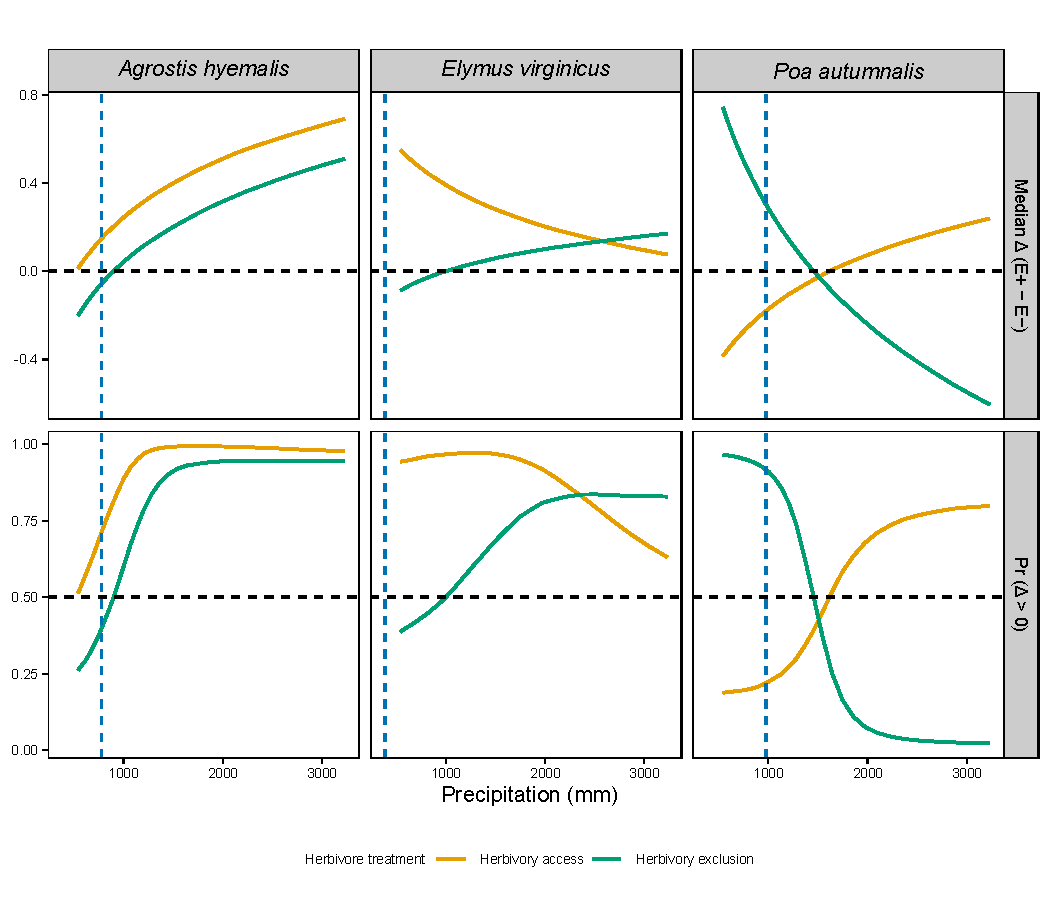
\includegraphics[width=1\linewidth]{../Figure/Growth_diff_stat.pdf}
		\caption{Effects of precipitation and endophyte presence on growth across three cool-season grass species. Lines show the predicted difference in growth between endophyte-present (E$^+$) and endophyte-absent (E$^-$) plants (Median $\Delta$, top row) and the posterior probability that this difference is positive (Pr($\Delta > 0$), bottom row) under fenced and unfenced treatments. Predictions were calculated at the 10th, 25th, 50th, 75th, and 90th percentiles of precipitation observed in the study. Horizontal dashed lines indicate $\Delta = 0$ (top row) and Pr($\Delta > 0$) = 0.5 (bottom row).}
		\label{sup:growth_delta}
\end{figure}

\begin{figure}[H]
		\centering
		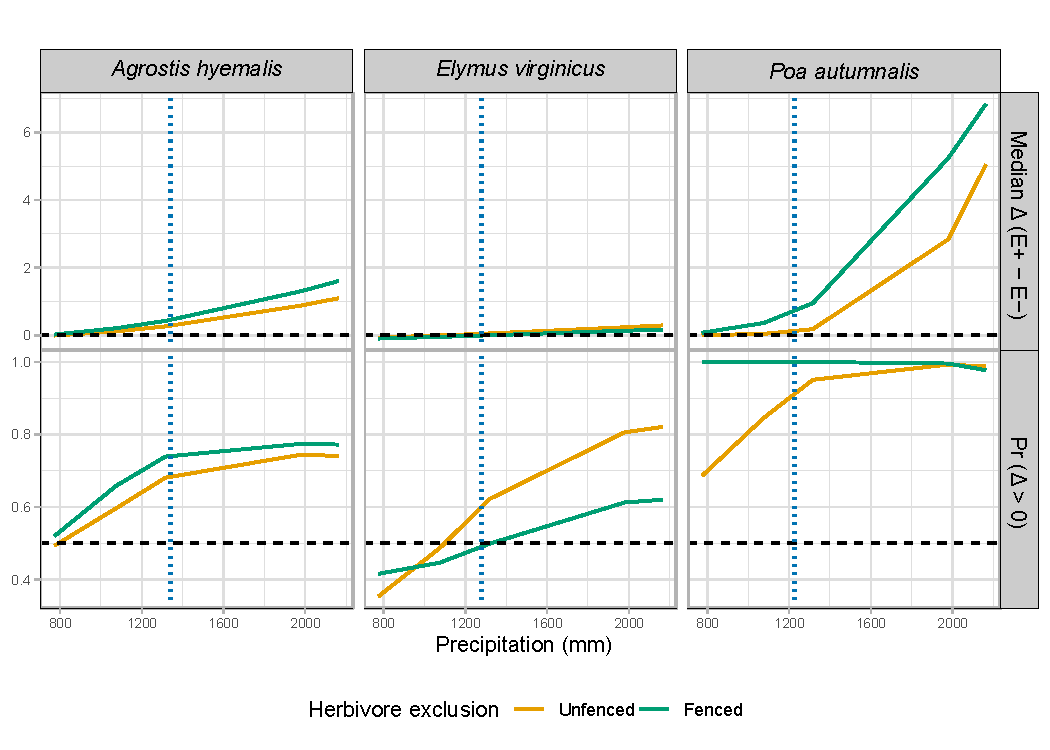
\includegraphics[width=1\linewidth]{../Figure/Flowering_diff_stat.pdf}
		\caption{Effects of endophyte infection on flowering output across a precipitation gradient for three cool-season grass species. Lines show the median posterior difference $\Delta$ (E$^{+}$ $-$ E$^{-}$) and the posterior probability that $\Delta > 0$ under fenced (herbivores excluded) and unfenced (herbivores present) conditions. Horizontal dashed lines indicate $\Delta = 0$ for median differences and $\mathrm{Pr}(\Delta > 0) = 0.5$. Endophyte effects were generally positive for \textit{Agrostis hyemalis} and \textit{Poa autumnalis}, but for \textit{Elymus virginicus} benefits were context-dependent, with costs at lower precipitation}
		\label{sup:flowering_delta}
\end{figure}


\begin{figure}[H]
		\centering
		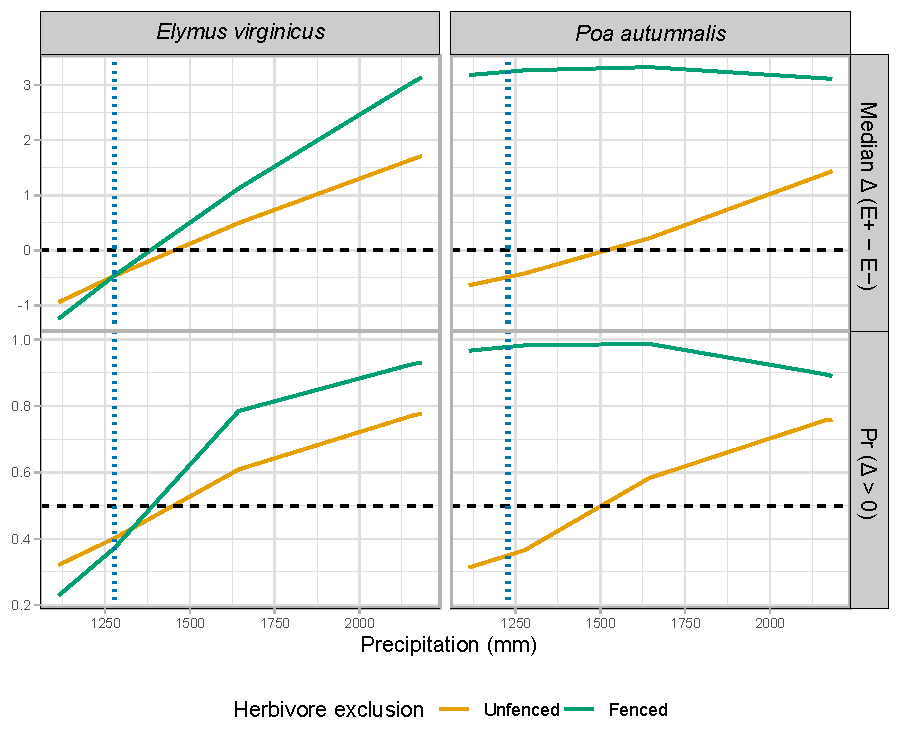
\includegraphics[width=1\linewidth]{../Figure/Spike_diff_stat.pdf}
		\caption{Effects of precipitation and endophyte presence on spike (reproductive output) for three cool-season grass species. Median $\Delta$ (E$^{+} - $E$^{-}$) and posterior probability $\mathrm{Pr}(\Delta > 0)$ are shown across precipitation quantiles. Herbivore exclusion treatments are indicated by color (Fenced = herbivores excluded, Unfenced = herbivores had access). Horizontal dashed lines indicate $\Delta = 0$ for medians and $\mathrm{Pr}(\Delta > 0) = 0.5$ for probabilities. Facets separate metrics and species.}
		\label{sup:spike_delta}
\end{figure}

%\begin{figure}[H]
%		\centering
%		
\includegraphics[width=0.50\linewidth]{ppt_surv_coeff.pdf}
%		\caption{Coefficient estimates from Bayesian models linking survival and geographic distance.
%		 Points represent posterior means and lines indicate 95\% credible intervals.
%		 Species abbreviations: \textit{Agrostis hyemalis} (AGHY), \textit{Elymus virginicus} (ELVI), and \textit{Poa autumnalis} (PAOU).
%		 Horizontal dashed lines denote zero effect.}
%		\label{Sup:temp_variation}
%\end{figure}
%
%\begin{figure}[H]
%		\centering
%		
\includegraphics[width=0.50\linewidth]{ppt_grow_coeff.pdf}
%		\caption{Coefficient estimates from Bayesian models linking growth and geographic distance.
%		 Points represent posterior means and lines indicate 95\% credible intervals.
%		 Species abbreviations: \textit{Agrostis hyemalis} (AGHY), \textit{Elymus virginicus} (ELVI), and \textit{Poa autumnalis} (PAOU).
%		 Horizontal dashed lines denote zero effect.}
%		\label{Sup:temp_variation}
%\end{figure}
%
%\begin{figure}[H]
%		\centering
%		
\includegraphics[width=0.50\linewidth]{ppt_flow_coeff.pdf}
%		\caption{Coefficient estimates from Bayesian models linking flowering and geographic distance.
%		 Points represent posterior means and lines indicate 95\% credible intervals.
%		 Species abbreviations: \textit{Agrostis hyemalis} (AGHY), \textit{Elymus virginicus} (ELVI), and \textit{Poa autumnalis} (PAOU).
%		 Horizontal dashed lines denote zero effect.}
%		\label{Sup:temp_variation}
%\end{figure}
%
%\begin{figure}[H]
%		\centering
%		
\includegraphics[width=0.50\linewidth]{ppt_spik_coeff.pdf}
%		\caption{Coefficient estimates from Bayesian models linking flowering and geographic distance.
%		 Points represent posterior means and lines indicate 95\% credible intervals.
%		 Species abbreviations: \textit{Agrostis hyemalis} (AGHY), \textit{Elymus virginicus} (ELVI), and \textit{Poa autumnalis} (PAOU).
%		 Horizontal dashed lines denote zero effect.}
%		\label{Sup:temp_variation}
%\end{figure}
%
%

%\begin{figure}[H]
%		\centering
%		\includegraphics[width=0.95\linewidth]{Figures/fig_pr_past_present_future.pdf}
%		\caption{Precipitation variation across the study sites from 1990 to 2100.
%		ds: Dormant season, dg: Growing season.}
%		\label{Sup:pr_variation}
%\end{figure}
%
%\begin{figure}[H]
%		\centering
%		\includegraphics[width=0.95\linewidth]{Figures/MIROC.pdf}
%		\caption{Past, Observed, present and future (MIROC Model) climate data across the study area.}
%		\label{Sup:projectionMIROC}
%\end{figure}
%
%\begin{figure}[H]
%		\centering
%		\includegraphics[width=0.99\linewidth]{Figures/ACCESS.pdf}
%		\caption{Past, Observed, present and future (ACCESS Model) climate data across the study area.}
%		\label{Sup:projectionACCESS}
%\end{figure}
%
%\begin{figure}[H]
%		\centering
%		\includegraphics[width=0.99\linewidth]{Figures/CESM1.pdf}
%		\caption{Past, Observed, present and future (CESM1 Model) climate data across the study area.}
%		\label{Sup:projectionCESM1}
%\end{figure}
%
%\begin{figure}[H]
%		\centering
%		\includegraphics[width=0.99\linewidth]{Figures/CMCC.pdf}
%		\caption{Past, Observed, present and future (CMCC Model) climate data across the study area.}
%		\label{Sup:projectionCMCC}
%\end{figure}
%
%\begin{figure}[H]
%		\centering
%		\includegraphics[width=0.959\linewidth]{Figures/site_year_weather.pdf}
%		\caption{Climate variation across the study sites during the monitoring period.}
%		\label{Sup:climate_variation}
%\end{figure}


\end{document}
